\documentclass[anon,12pt]{colt2019}
\usepackage[utf8]{inputenc}
\usepackage{mathtools, amsmath, amssymb, graphicx, verbatim}
%\usepackage[thmmarks, thref, amsthm]{ntheorem}
\usepackage{color}
\usepackage{wrapfig}
\usepackage{subcaption}
\usepackage[colorinlistoftodos,textsize=tiny]{todonotes} % need xargs for below
%\usepackage{accents}
\usepackage{bbm}
\usepackage{xspace}

\usetikzlibrary{calc}
\newcommand{\Comments}{1}
\newcommand{\mynote}[2]{\ifnum\Comments=1\textcolor{#1}{#2}\fi}
\newcommand{\mytodo}[2]{\ifnum\Comments=1%
  \todo[linecolor=#1!80!black,backgroundcolor=#1,bordercolor=#1!80!black]{#2}\fi}
\newcommand{\raf}[1]{\mynote{green}{[RF: #1]}}
\newcommand{\raft}[1]{\mytodo{green!20!white}{RF: #1}}
\newcommand{\jessie}[1]{\mynote{purple}{[JF: #1]}}
\newcommand{\jessiet}[1]{\mytodo{purple!20!white}{JF: #1}}
\newcommand{\bo}[1]{\mynote{blue}{[Bo: #1]}}
\newcommand{\botodo}[1]{\mytodo{blue!20!white}{[Bo: #1]}}
\ifnum\Comments=1               % fix margins for todonotes
  \setlength{\marginparwidth}{1in}
\fi


\newcommand{\reals}{\mathbb{R}}
\newcommand{\posreals}{\reals_{>0}}%{\reals_{++}}
\newcommand{\dom}{\mathrm{dom}}

\newcommand{\prop}[1]{\Gamma[#1]}
\newcommand{\eliccts}{\mathrm{elic}_\mathrm{cts}}
\newcommand{\eliccvx}{\mathrm{elic}_\mathrm{cvx}}
\newcommand{\elicpoly}{\mathrm{elic}_\mathrm{pcvx}}
\newcommand{\elicembed}{\mathrm{elic}_\mathrm{embed}}

\newcommand{\cell}{\mathrm{cell}}

\newcommand{\abstain}[1]{\mathrm{abstain}_{#1}}
\newcommand{\mode}{\mathrm{mode}}

\newcommand{\simplex}{\Delta_\Y}

% alphabetical order, by convention
\newcommand{\C}{\mathcal{C}}
\newcommand{\D}{\mathcal{D}}
\newcommand{\E}{\mathbb{E}}
\newcommand{\F}{\mathcal{F}}
\newcommand{\I}{\mathcal{I}}
\newcommand{\R}{\mathcal{R}}
\newcommand{\X}{\mathcal{X}}
\newcommand{\Y}{\mathcal{Y}}

\newcommand{\inprod}[2]{\langle #1, #2 \rangle}%\mathrm{int}(#1)}
\newcommand{\inter}[1]{\mathring{#1}}%\mathrm{int}(#1)}
%\newcommand{\expectedv}[3]{\overline{#1}(#2,#3)}
\newcommand{\expectedv}[3]{\E_{Y\sim{#3}} {#1}(#2,Y)}
\newcommand{\toto}{\rightrightarrows}
\newcommand{\strip}{\mathrm{strip}}
\newcommand{\trim}{\mathrm{trim}}
\newcommand{\fplc}{finite-piecewise-linear and convex\xspace} %xspace for use in text
\newcommand{\conv}{\mathrm{conv}}
\newcommand{\ones}{\mathbbm{1}}
\DeclarePairedDelimiter\ceil{\lceil}{\rceil}

\newcommand{\Ind}{\mathbf{1}}

\DeclareMathOperator*{\argmax}{arg\,max}
\DeclareMathOperator*{\argmin}{arg\,min}
\DeclareMathOperator*{\arginf}{arg\,inf}
\DeclareMathOperator*{\sgn}{sgn}

%\newtheorem{theorem}{Theorem}
%\newtheorem{lemma}{Lemma}
%\newtheorem{proposition}{Proposition}
%\newtheorem{definition}{Definition}
%\newtheorem{corollary}{Corollary}
%\newtheorem{conjecture}{Conjecture}


\title{Convex Surrogates via Polyhedral Losses}
\coltauthor{%
 \Name{Jessie} \Email{email}\\
 \addr CU
 \AND
 \Name{Raf} \Email{email}\\
 \addr CU
 \AND
 \Name{Bo}  \Email{email}\\
 \addr MSFT
}

\begin{document}

\maketitle

\begin{abstract}
  \bo{TODO - iterate!}
  Convex surrogates are sweet.
  Given a loss for a classification-like problem, there are two natural approaches to design convex surrogates.
  First, one may attempt to map each prediction to a low-dimensional vector, and try to find a convex loss in that space with the right calibration.
  Second, one may simply try to find a surrogate within the class of piecewise-linear convex, or polyhedral, losses.
  We show an equivalence between these two approaches, and \raf{more stuff}.
  We show that every loss with a finite number of predictions has a convex surrogate in the above sense using one fewer dimension that the number of outcomes, and give a full characterization of the losses needing only $d$ dimensions for such a surrogate.
  We then apply this characterization to show novel lower bounds for abstain loss, demonstrating the power of our techniques over \raf{check this} alternatives such as feasible subspace dimension.
\end{abstract}
\begin{keywords}%
  information elicitation, proper scoring rules, surrogate loss functions
\end{keywords}

\section{Introduction}\label{sec:intro}

\raf{MOVED FROM SEC 2; maybe incorporate?}
Often, for computational or other reasons, one is interested in a property $\gamma$ such as the mode, but wishes to elicit it by minimizing some other ``surrogate'' loss $L$ over some other space such as $\reals^d$, then mapping the result back to $\R$ using a link function.
We now formalize this procedure.


Convex surrogate losses are a central building block in machine learning for classification and classification-like problems.
A growing body of research is concerned with designing and analyzing convex surrogates for given loss functions, and more broadly, understanding when such surrogates can and cannot be found.\raf{cite}
For example, recent work has developed tools to bound the required number of dimensions of the surrogate's hypothesis space. (\cite{frongillo2015elicitation,  ramaswamy2016convex}) \raf{cite}
Yet in some cases these bounds are far from tight, such as for \emph{abstain loss} (classification with an abstain option)~(\cite{bartlett2008classification, yuan2010classification, ramaswamy2016convex, ramaswamy2018consistent})\raft{cite}.
Furthermore, the kinds of strategies available for constructing surrogates, and their relative power, are not well-understood.

We augment this literature by studying a particularly natural approach for finding convex surrogates, wherein one \emph{embeds} a discrete loss function into a real vector space so that it can be convexified.
Special cases include hinge loss as a surrogate for 0-1 loss and the abstain surrogate mentioned above.~\cite{crammer2001algorithmic}\raft{cite}
\bo{it felt like the following results were only a warmup instead of main results. Not sure how to change this, maybe a paragraph break helps.}

Using tools from property elicitation, we show a tight relationship between such embeddings and the class of polyhedral (i.e.\ piecewise-linear convex) loss functions: whenever such an embedding is possible, the discrete loss can be convexified into a polyhedral loss, and moreover, every polyhedral loss function is the result of such an embedding of some discrete loss.

We go on to study the \emph{embedding dimension}: the minimal dimension for a given loss to be so embedded.
Our results give a complete characterization in the case of dimension 1 (real-valued surrogates):
a discrete loss can be embedded in the real line if and only if it is order-sensitive, meaning there is an ordering of the predictions such that the loss increases as one moves away from the correct prediction.
We show further that order-sensitivity characterizes a much broader condition: the existence of any real-valued convex surrogate.
In other words, in one dimension the embedding approach to surrogate construction loses no generality.
In higher dimensions, we give a characterization of embeddability in terms of convex polytopes, which yields tight bounds for abstain loss.
We conclude with several conjectures and directions for future work.

\subsection{Related works}
Convex surrogates have been formalized and investigated in a variety of past work such as \citet{crammer2001algorithmic,bartlett2006convexity,bartlett2008classification}, particularly in the context of $0-1$ loss, distributions on just two outcomes, and support vector machines.
%  \cite{crammer2001algorithmic} is one of the first papers to present a convex surrogate for multiclass classification problems in the context of support vector machines.
%  They use the convex surrogate $L(\textbf{r},y) = (\max_{j\neq y} r_j - r_y + 1)_+$, where $\textbf{r}$ is a $n$-dimensional vector corresponding to the entire distribution, and $r_j$ is the $j^{th}$ component of \textbf{r}.
%
%  \cite{bartlett2006convexity} provides one of the most well-known formalizations of convex surrogates for properties on binary outcomes.
%  This work evaluates the risk bounds of convex surrogates and shows the sufficiency of convex surrogates such as logistic loss to replace the 0-1 loss for ease of optimization, and has inspired a line of research in the design of consistent surrogate losses for binary classification problems.
%  \jessiet{This is based on what I remember.  Couldn't find the free version (off the campus network) but also didn't look hard at all, since I'm guessing one of you two already knows this paper better than I do.}
%
%%  \cite{bartlett2008classification} studies the abstain property with $n=2$ and shows a variation of the hinge loss that is one convex surrogate that elicits the abstain property to two outcomes.
%
%  \cite{ramaswamy2012classification} discuss and formalize the notion of \emph{convex calibration} dimension for finite properties.
%  The concept they call convex calibration dimension is one notion of elicitation complexity discussion in this paper.
%  Denoted here by $\eliccvx(\gamma)$, convex calibration refers to the minimum dimension $d$ such that the property $\gamma$ can be indirectly elicited by a convex loss $L:\reals^d \to \reals^\Y_+$.
%
%  Most of the preliminary work on the construction of convex surrogate losses focuses on learning the mode in a binary classification problem.
  One of the first works formally studying convex surrogates beyond binary outcomes is~\cite{ramaswamy2018consistent} (originally 2014), who give an embedding of the \emph{abstain loss} into very few dimensions.
For the case of $\reals^2$, we will show that no embedding can do better.
%  Rather than focusing on the mode, this paper proves bounds on the elicitation complexity of the abstain property.
%  They provide a consistent surrogate that elicits abstain with $\alpha = 1/2$ in $\ceil*{\log_2 n}$ dimensions. \jessiet{I don't like how much I'm talking about elicitation without the context.}
%  It remains unknown if this bound is tight, although in Conjecture~\ref{conj:abstain-tight}, we conjecture that it is, at least from the perspective from ``embedding''.
%  If true, then we will need new approaches in order to indirectly elicit the abstain property by a convex surrogate for any dimension lower than $\ceil*{\log_2 n}$.
%
%  \cite{agarwal2015consistent} introduces the notion of a \emph{calibrated property}, which is very similar to our \emph{surrogate property} that we elicit by a convex surrogate in lieu of directly eliciting a finite property.
%  However, they do not consider properties to be set-valued, leading to subtle differences in the property values for some distributions.
%  Additionally, most of their results focus on linear properties. \jessiet{is there a relationship between linear and orderable properties?  If not, we can probably remove this statement.}
%
  \cite{agarwal2015consistent} and ~\cite{ramaswamy2016convex} study the existence of convex surrogates; the latter proves lower bounds on dimensionality of hypothesis spaces for e.g. $0-1$ loss via their notion of feasible subspace dimension.
  These works are generally not directly comparable to our results, as they do not consider the embedding method.
  However, we will mention relevant results inline.
%  In~\cite{ramaswamy2016convex}, the authors introduce a new method of obtaining upper bounds on elicitation complexity called the \emph{Feasible Subspace Dimension}.
%  This method uses local information about distributions in a property in order to find bounds on the convex elicitation complexity of a property.
%  For example, Feasible Subspace Dimension can be used to find a tight bound on $\eliccvx$(mode), but does not reveal a tight bound for the abstain property discussed later.
%  This suggests that the bound on $\eliccvx$(abstain) must be found using more \emph{global} information about the property.
%  We discuss this in Section~\ref{sec:general-dimensions}, showing previously unknown necessary conditions for embedding finite properties.


\subsection{Notation}
\begin{itemize}
  \item $\Y$ is the finite outcome space, and $n := |\Y|$.
  \item $\simplex\subseteq\reals^\Y$ is the set of distributions over $\Y$, thought of as vectors of probabilities.
  \item For an outcome $y$, we denote $p_y$ as the probability of outcome $y$ being observed in nature.
  \item If $\gamma = \prop{\ell}$, then $\gamma:\simplex \toto \R$ is the property elicited by the loss $\ell: \R \to \reals^\Y$.
  \item $d$ is the dimension of the embedding space
  \item $L:\reals^d \to \reals^\Y_+$ is a loss taking a report $u \in \reals^d$ and mapping the loss over each outcome in $\Y$. \raf{Changed to $\reals^\Y_+$ below.}
  \item $\Gamma: \simplex \toto \reals^d$ is the set-valued property mapping a probability distribution to a report $u \in \reals^d$.
  \item $\Gamma_u = \{ p \in \simplex : u \in \Gamma(p) \}$
  \item $\psi$ is the link function (see below)
  \item $\varphi:\R \to \reals^d$ is the embedding function
  \item $\trim(\Gamma)$ and $\strip(\Gamma)$
  \item $\eliccvx$, $\elicembed$, and $\elicpoly$
  \item $V$ and $B(P)$ as we get ready for later.
\end{itemize}

\section{Setting and Background}

While we have motivated our study in terms of a given discrete loss function, essentially all of our results instead work with the \emph{property} this loss elicits: the map from the outcome distribution to the set of reports (predictions) which optimize the expected loss.
Thus, throughout the paper, our central object of study will be \emph{finite elicitable properties}, which as above map distributions to reports from a finite set, and ignore the loss.
In this way, we can leverage the large body of work on property elicitation.
We begin with the relevant definitions and notation.

Let $\Y$ be a finite outcome (label) space, and throughout let $n=|\Y|$.
The set of probability distributions on $\Y$ is denoted $\simplex\subseteq\reals^{\Y}$, represented as vectors of probabilities.
We write $p_y$ for the probability of outcome $y \in \Y$ drawn from $p \in \simplex$.

We write loss functions as $L:\R\to\reals^\Y_+$ which map a report (prediction) $r\in\R$ to the vector of loss values $L(r) = (L(r)_y)_{y\in\Y}$ for each possible outcome $y\in\Y$.
Often $\R$ will be taken to be a finite set for the given discrete loss (in which case we will write $\ell$ not $L$), and $\reals^d$ for the surrogate.
The expected loss of report $r$ when $y \sim p$ is written $\inprod{p}{L(r)}$.
For example, 0-1 loss is a discrete loss with $\R = \Y = \{-1,1\}$ given by $\ell(r)_y = \Ind[r \neq y]$.
Two important examples of surrogates for 0-1 loss, with $\R=\reals$, are hinge loss $L(u)_y = \max(0,1-yu)$ and logistic loss $L(u)_y = \log(1+\exp(-yu))$.

To formalize and study the relationship between the given loss and its surrogate, we adopt terminology from the property elicitation literature, which elevates the \emph{property}, or map from distributions to optimal reports, as a central object to study in its own right.
In the case of discrete losses, this map is multivalued, meaning a single distribution could map to multiple optimal reports.
(For example, when $p=(1/2,1/2)$, both $y=1$ and $y=-1$ optimize 0-1 loss.)
To this end, we will use double arrow notation to mean a mapping to all nonempty subsets, so that $\gamma: \simplex \toto \R$ is shorthand for $\gamma: \simplex \to 2^{\R} \setminus \emptyset$.

\begin{definition}[Property, level set]\label{def:property}
  A \emph{property} is a function $\Gamma:\simplex\toto\R$.
  The \emph{level set} of $\Gamma$ for report $r$ is the set $\Gamma_r := \{p : r \in \Gamma(p)\}$.
\end{definition}

\begin{definition}[Finite property, non-redundant]
  A property $\Gamma:\simplex\toto\R$ is \emph{redundant} if for some $r,r'\in\R$ we have $\Gamma_r \subseteq \Gamma_{r'}$, and \emph{non-redundant} otherwise.
  $\Gamma$ is \emph{finite} if it is non-redundant and $\R$ is a finite.
  We typically write finite properties in lower case, as $\gamma$.
\end{definition}

Thus, $\Gamma(p)$ is the set of reports which should be optimal for a given distribution $p$, and $\Gamma_r$ is the set of distributions for which the report $r$ should be optimal.
For example, the \emph{mode} is the property $\mode(p) = \argmax_{y\in\Y} p_y$, which is finite.
The mode captures the set of optimal reports for 0-1 loss: for each distribution over the labels, one should report the most likely label.
In this case we say 0-1 loss \emph{elicits} the mode, as we formalize below.
This terminology comes from the information elicitation literature~\citep{savage1971elicitation,osband1985information-eliciting,lambert2008eliciting}, in which a report $r$ is elicited from some forecaster by scoring her with a loss on the observed outcome $y$.

\begin{definition}[Elicits]
  A loss $L:\R\to\reals^\Y_+$, \emph{elicits} a property $\Gamma:\simplex \toto \R$ if
  \begin{equation}
    \forall p\in\simplex,\;\;\;\Gamma(p) = \argmin_{r \in \R} \inprod{p}{L(r)}~.
  \end{equation}
  As $\Gamma$ is uniquely defined by $L$, we write $\prop{L}$ to refer to the property elicited by a loss $L$.
\end{definition}

For finite properties and discrete losses, we will use lowercase notation $\gamma$ and $\ell$, respectively, while $\Gamma$ and $L$ will be used for general properties.
Often we will work with two properties simultaneously, a finite property $\gamma:\simplex\toto\R$, and its embedded version $\Gamma:\simplex\toto\reals^d$.
In this case, we write the embedded reports as $u\in\reals^d$, reserving $r\in\R$ for the finite property.

Most of the loss functions $L$ we consider will be piecewise linear and convex, or \emph{polyhedral}; we therefore will make use of the theory of convex polytopes.
In $\reals^d$, a \emph{polyhedral set} or \emph{polyhedron} is the intersection of a finite number of halfspaces.
A \emph{polytope} is a bounded polyhedral set.
A convex function $f:\reals^d\to\reals$ is \emph{polyhedral} if its epigraph is polyhedral, or equivalently, if it can be written as a pointwise maximum of a finite set of affine functions~\cite{rockafellar1997convex}.

\begin{definition}[Polyhedral loss]
  A loss $L: \reals^d \to \reals^{\Y}_+$ is a \emph{polyhedral} if $L(u)_y$ is a polyhedral (convex) function of $u$ for each $y\in\Y$.
\end{definition}
For example, note that hinge loss is polyhedral, as is the surrogate for abstain loss described in \S~\ref{sec:important-examples}.

\subsection{Link Functions and Elicitation Complexity}\label{sec:link-elic}

When designing a surrogate loss function, we require some sort of statistical consistency with the original loss, so that minimizing the surrogate is an effective alternative to directly minimizing the original loss.
We formalize this consistency below in terms of the properties elicited by each loss.
In particular, we seek a \emph{link} function, which maps optimal reports from the surrogate to the original reports, satisfying certain guarantees.
\bo{Maybe mention that previous formalizations are for single-valued properties only if true? And if so, that they don't really apply to finite properties??}

\begin{definition}[Calibrated Link]\label{def:links}
  Let properties $\gamma:\simplex\toto\R$ and $\Gamma:\simplex\toto\R'$ be given.
  A \emph{link function} is a map $\psi:\R'\to\R$.
  We say that a link $\psi$ is:
  \begin{itemize}
  \item \emph{Calibrated} if for all $p\in\simplex$, $r'\in \Gamma(p) \implies \psi(r') \in \gamma(p)$; in other words, if for all $r'\in\R'$, $\Gamma_{r'} \subseteq \gamma_{\psi(r')}$;
  \item \emph{Separated}, with respect to a loss $L$ eliciting $\Gamma$, if for all $p \in \simplex$,
  \begin{align*}
  \inf_{u \in \R'; \psi(u) \not \in \gamma(p)} \E_{Y\sim p}[L(u, Y)] > \inf_{u \in \R'}\E_{Y\sim p}[L(u, Y)]~.
  \end{align*}
  \end{itemize}
\end{definition}

Roughly speaking, a calibrated link requires that optimal surrogate reports map to optimal original reports, while a separated link adds the stronger guarantee that one cannot approach the optimal surrogate loss while making suboptimal original predictions.
A classic example of a link which is both calibrated and separated is $\psi = \sgn$ when $\gamma=\mode$ and $L$ is either hinge loss or logistic loss.
On the other hand, the link $\psi(u) =
\begin{cases}
  -1 & u \leq -1\\
  1 & u > -1
\end{cases}$
would not be separated for hinge loss, but it would still be calibrated, as the reports $u\in(-1,1)$ are optimal for hinge loss only when $p=(1/2,1/2)$, in which case both $-1$ and $1$ are optimal for the mode (0-1 loss).

\raft{Aside about other link definitions commented out}
% As a brief aside, it is interesting to contrast the definitions above with the following: a link is
% \emph{exhaustive} if for all $p\in\simplex$, $\gamma(p) = \psi(\Gamma(p)) := \{\psi(r') : r'\in\Gamma(p)\}$.
% A \emph{strong link} is a set-valued function $\psi:\R'\toto\R$ such that for all $p\in\simplex$ and $r'\in\R'$, we have $r'\in\Gamma(p) \implies \gamma(p) = \psi(r')$.
% If sign is interpreted as set-valued (0 maps to $\{1,-1\}$, then it is strong for logistic.  If not, sign is not exhaustive for logistic.  Sign is exhaustive for hinge.}

It is often useful to express the relationship between $L$ and $\gamma$ above directly, which is the notion of \emph{indirect elicitation}.

\begin{definition}
  A loss \emph{indirectly elicits} a property $\gamma$ if it elicits a property with a calibrated link to $\gamma$.
\end{definition}

Often one is given a property $\gamma$ (typically via a discrete loss $\ell$) and one seeks a surrogate loss $L$ with certain attributes, such as convexity, smoothness, etc.
In doing so, we may be interested in the minimum number of dimensions needed for such an indirect elicitation scheme; this is the notion of \emph{elicitation complexity}~\citep{lambert2008eliciting,fissler2016higher,frongillo2015elicitation}.
The two notions of elicitation complexity we use most are as follows: let $\eliccvx(\gamma)$ be the minimum dimension $d$ such that $\gamma$ can be indirectly elicited by a convex loss function $L: \R'^d \to \reals^\Y_+$, and $\elicpoly(\gamma)$ the minimum such $d$ where $L$ is polyhedral.
We will also discuss $\eliccts$, which is the complexity with respect to continuous, real-valued, non-locally-constant properties (\S~\ref{sec:1d}), and $\elicembed$, which is the minimum dimension for $\gamma$ to be embedded (Definition~\ref{def:embedding-dim}).

As a brief aside, we note that previous definitions of elicitation complexity have used a more straightforward link function, as the properties considered were single-valued~\citep{lambert2008eliciting,fissler2016higher,frongillo2015elicitation}.
In particular, if both $\gamma$ and $\Gamma$ are single-valued, these works simply require $\gamma = f \circ \Gamma$.
When $\Gamma$ is set-valued, one still straightforwardly requires $\gamma(p) = f(u)$ for all $u \in \Gamma(p)$.
The notion a calibrated link from Definition~\ref{def:links} is only required when both $\gamma$ and $\Gamma$ could be set-valued, as is the case in general for convex surrogates of finite properties.


\subsection{Important Examples}\label{sec:important-examples}
  Ranking and classification problems are well-known to the field of machine learning.
  The most studied classification problem is the elicitation of the mode.
  While the mode over $n$ outcomes is elicitable by 0-1 loss, it is known that eliciting the mode by a convex loss is much more difficult.
  In fact, the best convex surrogate that can be used to elicit the mode ``embeds'' the reports into $\reals^{n-1}$.
  Therefore, we say $\eliccvx($mode$) = n-1$.

  A property of interest similar to the mode is the $\abstain{\alpha}$ property.
  In this property in which one reports the most likely outcome if the probability of such an outcome is greater than $1-\alpha$, and otherwise ``abstains'' from reporting.
  That is, $\gamma(p) = \argmax_{r \in \R}p_r$ if $\max_{r \in \R} p_r \geq 1-\alpha$ and is ``abstain'' otherwise.

  The finite loss eliciting $\alpha$ can be written
  $\ell(r,y) = \begin{cases}
  0 & r = y\\
  \alpha & r = \text{abstain}\\
  1 & r \neq y, r \neq \text{abstain}\\
  \end{cases}$.

\cite{ramaswamy2018consistent} show that $\elicpoly(\abstain{1/2}) \leq \ceil{\log_2 n}$, although it is not known if this bound is tight.


\section{Polyhedral Losses and Embeddings}
\label{sec:poly-loss-embed}

For many problems in machine learning, researchers have naturally converged on some notion of learning a finite property by ``embedding'' the possible labels or predictions into $\reals^d$ and minimizing a consistent convex surrogate loss.
Here, we formalize a notion of embedding which captures these techniques, and show some geometric and topological characteristics of embeddable properties.

\begin{definition}
  A property $\Gamma : \simplex \toto \reals^d$ \emph{embeds} a property $\gamma : \simplex \toto \R$ if there exists some injective embdedding $\varphi:\R\to\reals^d$ such that for all $p\in\simplex,r\in\R$ we have $r \in \gamma(p) \iff \varphi(r) \in \Gamma(p)$.
  Similarly, we say a loss $L:\reals^d\to\reals^\Y$ embeds $\gamma$ if $\prop{L}$ embeds $\gamma$.
\end{definition}

In this section, we focus on the structure of embeddable properties, and what a property embedding another must look like.
In the following sections, however, we will focus on the dimension $d$, and ask questions about the minimum $d$ required to embed a property.

\begin{definition}\label{def:embedding-dim}
  We say $\gamma$ is \emph{$d$-embeddable}, or just \emph{embeddable}, if such an $L$ exists and is convex.
  The \emph{embedding dimension} of a finite property $\gamma$, written $\elicembed(\gamma)$, is the minimum $d\geq 0$ such that $\gamma$ is $d$-embeddable.
\end{definition}

When working with convex losses which are not strictly convex, one quickly encounters redundant properties: if $\inprod{p}{L(\cdot)}$ is minimized by a point where $p\cdot L$ is flat, then there will be an uncountable set of reports which also minimize the loss.
As results in property elicitation typically assume non-redudant properties (e.g.~\cite{frongillo2014general,frongillo2015elicitation}) it is useful to consider a transformation which removes redundant level sets.
We capture this transformation as the trim operator presented below.

\begin{definition}\label{def:trim}
  Given an elicitable property $\Gamma:\simplex \toto\R$, we define $\trim(\Gamma) = \{\Gamma_u : u \in \R \text{ s.t. } \forall u'\in\R,u'\neq u,\, \Gamma_u \not\subseteq \Gamma_{u'}\}$ as the set of maximal level sets of $\Gamma$.
\end{definition}
\raft{Note for later: should be able to show that the union of trim is the simplex.}

Take note that the unlabeled property $\trim(\Gamma)$ is non-redundant, meaning that for any $\theta \in \trim(\Gamma)$, there is no level set $\theta' \in \trim(\Gamma)$ such that $\theta \subset \theta'$.

Before we state our first result, we will need to general lemmas about properties and their losses.
The first follows from standard results relating finite properties to power diagrams (see Theorem~\ref{thm:aurenhammer} in the appendix), and its proof is omitted.
The second is closely related to the trim operator: it states that if some subset of the reports are always represented among the minimizers of a loss, then one may remove all other reports and elicit the same property (with those other reports removed).

\begin{lemma}\label{lem:finite-full-dim}
  Let $\gamma$ be a finite (non-redundant) property elicited by a loss $L$.
  Then the negative Bayes risk $G$ of $L$ is polyhedral, and the level sets of $\gamma$ are the projections of the facets of the epigraph of $G$ onto $\simplex$, and thus form a power diagram.
  In particular, the level sets $\gamma$ are full-dimensional in $\simplex$ (i.e.,\ of dimension $n-1$).
\end{lemma}

\begin{lemma}\label{lem:loss-restrict}
  Let $L$ elicit $\Gamma:\simplex\toto\R_1$, and let $\R_2\subseteq\R_1$ such that $\Gamma(p) \cap \R_2 \neq \emptyset$ for all $p\in\simplex$.
  Then $L|_{\R_2}$ ($L$ restricted to $\R_2$) elicits $\gamma:\simplex\toto\R_2$ defined by $\gamma(p) = \Gamma(p)\cap \R_2$.
  Moreover, the Bayes risks of $L$ and $L|_{\R_2}$ are the same.
\end{lemma}
\begin{proof}
  Let $p\in\simplex$ be fixed throughout.
  First let $r \in \gamma(p) = \Gamma(p) \cap \R_2$.
  Then $r \in \Gamma(p) = \argmin_{u\in\R_1} \inprod{p}{L(u)}$, so as $r\in\R_2$ we have in particular $r \in \argmin_{u\in\R_2} \inprod{p}{L(u)}$.
  For the other direction, suppose $r \in \argmin_{u\in\R_2} \inprod{p}{L(u)}$.
  By our assumption, we must have some $r^* \in \Gamma(p) \cap \R_2$.
  On the one hand, $r^*\in\Gamma(p) = \argmin_{u\in\R_1} \inprod{p}{L(u)}$.
  On the other, as $r^* \in \R_2$, we certainly have $r^* \in \argmin_{u\in\R_2} \inprod{p}{L(u)}$.
  But now we must have $\inprod{p}{L(r)} = \inprod{p}{L(r^*)}$, and thus $r \in \argmin_{u\in\R_1} \inprod{p}{L(u)} = \Gamma(p)$ as well.
  We now see $r \in \Gamma(p) \cap \R_2$.
  Finally, the equality of the Bayes risks $\min_{u\in\R_1} \inprod{p}{L(u)} = \min_{u\in\R_2} \inprod{p}{L(u)}$ follows immediately by the above, as $\emptyset \neq \Gamma(p)\cap\R_2 \subseteq \Gamma(p)$ for all $p\in\simplex$.
\end{proof}

We now state our first result, which shows remarkable structure of embeddable properties, and the properties that embed them.
First, we conclude that any embeddable property must be elicitable.
We also conclude that if $\Gamma$ embeds $\gamma$, the level sets of $\Gamma$ must all be redundant relative to $\gamma$.
In other words, $\Gamma$ is exactly the property $\gamma$, just with other reports filling in the gaps between the embedded reports of $\gamma$.
(When working with convex losses, these extra reports are typically the convex hull of the embedded reports.)
In this sense, we can regard embedding as a minor departure from direct elicitation: if a loss $L$ elicits $\Gamma$ which embeds $\gamma$, we can think of $L$ as essentially eliciting $\gamma$ itself.
Finally, we have an important converse: if $\Gamma$ has finitely many full-dimensional level sets, or if $\trim(\Gamma)$ is finite, then $\Gamma$ must embed some finite elicitable property with those same level sets.
\raft{Commented out what used to be before trim; not 100\% sure how to integrate.}
% Looking at the $\trim$ of a property allows us to relate the finite property of interest to the subtlely different surrogate property that we actually elicit when embedding the original property into $\reals^d$.
% In the surrogate property, there is often an infinite set of ``hidden'' level sets corresponding to the reports in the convex hull of embedded points whose level sets have nonempty intersection.
% Taking the $\trim$ thus allows us to remove labels so that we can relate the optimal sets of original reports and their embedded points, and then we remove the ``hidden'' level sets that are only optimal when we are indifferent between a subset of the embedded points.


\begin{proposition}\label{prop:embed-trim}
  Let $\Gamma:\simplex\toto\reals^d$ be an elicitable property.
  The following are equivalent:
  \begin{enumerate}
  \item $\Gamma$ embeds a finite property $\gamma:\simplex \toto \R$.
  \item $\trim(\Gamma)$ is a finite set, and $\cup\,\trim(\Gamma) = \simplex$.
  \item There is a finite set of full-dimensional level sets $\Theta$ of $\Gamma$, and $\cup\,\Theta = \simplex$.
  \end{enumerate}
  Moreover, when any of the above hold, $\{\gamma_r : r\in\R\} = \trim(\Gamma) = \Theta$, and $\gamma$ is elicitable.
\end{proposition}
\begin{proof}
  Let $L$ elicit $\Gamma$.

  1 $\Rightarrow$ 2:
  By the embedding condition, taking $\R_1 = \reals^d$ and $\R_2 = \varphi(\R)$ satisfies the conditions of Lemma~\ref{lem:loss-restrict}: for all $p\in\simplex$, as $\gamma(p) \neq \emptyset$ by definition, we have some $r\in\gamma(p)$ and thus some $\varphi(r) \in \Gamma(p)$.
  Let $G(p) := -\min_{u\in\reals^d} \inprod{p}{L(u)}$ be the negative Bayes risk of $L$, which is convex, and $G_{\R}$ that of $L|_{\varphi(\R)}$.
  By the Lemma, we also have $G = G_\R$.
  As $\gamma$ is finite, $G$ is polyhedral.
  Moreover, the projection of the epigraph of $G$ onto $\simplex$ forms a power diagram, with the facets projecting onto the level sets of $\gamma$, the cells of the power diagram.
  (See Theorem~\ref{thm:aurenhammer}.)
  As $L$ elicits $\Gamma$, for all $u\in\reals^d$, the hyperplane $p\mapsto \inprod{p}{L(u)}$ is a supporting hyperplane of the epigraph of $G$ at $(p,G(p))$ if and only if $u\in\Gamma(p)$.
  This supporting hyperplane exposes some face $F$ of the epigraph of $G$, which must be contained in some facet $F'$.
  Thus, the projection of $F$, which is $\Gamma_u$, must be contained in the projection of $F'$, which is a level set of $\gamma$.
  We conclude that $\Gamma_u \subseteq \gamma_r$ for some $r\in\R$.
  Hence, $\trim(\Gamma) = \{\gamma_r : r\in\R\}$, which is finite, and unions to $\simplex$.


  %%% The below is basically the argument from the Lemma, for this specific case.
  % We will first show $L'$ elicits $\gamma$, where $L':\R\to\reals^\Y_+$ is defined by $L'(r) = L(\varphi(r))$.
  % From the definition of embedding, for all $p\in\simplex$ we have $r \in \gamma(p) \iff \varphi(r) \in \Gamma(p) = \argmin_{u\in\reals^d} p\cdot L(u)$.
  % Thus, $r\in\gamma(p)$ implies $r \in \argmin_{r'\in\R} p\cdot L(\varphi(r')) = \argmin_{r'\in\R} p\cdot L'(r')$.
  % For the other direction, let $r \in \argmin_{r'\in\R} p\cdot L'(r')$, and let $r'\in\gamma(p)$ (where use $\gamma(p) \neq \emptyset$).
  % By the above, we have $r'\in\argmin_{r'\in\R} p\cdot L'(r')$ as well, so we must have $p\cdot L'(r) = p\cdot L'(r')$, and therefore $p\cdot L(\varphi(r)) = p\cdot L(\varphi(r'))$.
  % But we also have $\varphi(r') \in \argmin_{u\in\reals^d} p\cdot L(u)$, and therefore $\varphi(r) \in \argmin_{u\in\reals^d} p\cdot L(u) = \Gamma(p)$.
  % By the definition of embedding, we now have $r \in \gamma(p)$, as was to be shown.

  % for all the given that $\Gamma$ embeds the finite property $\gamma$, we show that $\trim(\Gamma) = \{\Gamma_u : u \in \varphi(\R) \} = \{\gamma_r : r \in \R\}$.
  % By elicitability, each level set $\Gamma_u$ corresponds to a subgradient of the expected score function, call it $G(p) := -\langle p, L(\Gamma(p))\rangle$ for any choice from $\Gamma$.
  % We claim $G$ is polyhedral. $\gamma$ is finite (and by definition non-redundant), so each level set $\gamma_r = \Gamma_{\phi(r)}$ is full-dimensional\bo{need to prove this separately in a lemma}.
  % So the corresponding subgradient is tangent to $G$ above a full-dimensional level set, and this is true for every $\gamma_r$.
  % Every $p$ is in one of these level sets and so is below some facet.
  % This implies that $G$ is polyhedral with facets exactly corresponding to $\{\gamma_r : r \in \R\} = \{\Gamma_u : u \in \varphi(\R)\}$.
  % Finally, for any $u \not\in \varphi(\R)$, we have\bo{need to cite a lemma statement, per discussion with Raf} that $\Gamma_u$ lies below some face of the epigraph of $G$, hence is contained in the set lying below some facet, which is one of the $\Gamma_{\varphi(r)}$.
  % So the maximal level sets of $\Gamma$ are exactly those lying below facets, which are exactly the level sets of $\gamma$.
  % This gives 2, and the fact that the level sets of $\gamma$ are full-dimensional and union to $\Delta_{\Y}$ gives 3.

  % Clearly, $\trim(\Gamma) \supseteq \{\Gamma_u : u \in \varphi(\R)\}$ as we are simply restricting the number of level sets we are indexing over.
%  Now, consider some $\theta \in \trim(\Gamma)$ and the report $u$ so that $\theta = \Gamma_u$.
%  If $u \in \varphi(\R)$, then clearly we are done.
%  If $u \not\in \varphi(\R)$ but there is some report $w \in \varphi(\R)$ so that $\Gamma_u = \Gamma_w$, then we are again done since $\trim(\Gamma)$ is non-redundant.
%  If there is no such $w \in \R$, then we claim $\Gamma_u \not \in \trim(\Gamma)$.
%  To see this, consider that if $\Gamma_u$ is full-dimensional, it must be a relabeling of another report by Lemma~\ref{lem:unique-opt-on-inter} in the Appendix.
%  If $\Gamma_u$ is not full-dimensional, it must be a proper subset of some full-dimensional level set by Lemma~\ref{lem:trim-subsets-not-full-dimensional}, and therefore not in $\trim(\Gamma)$.
%%\jessiet{skimmed over this, but follows from the convexity of the scoring rule.  My thought for the paper is to put that proof in the appendix,and just have a footnote or side note here with a reference to the proof in the appendix.}
%  Thus, we conclude $\trim(\Gamma) \subseteq \{\Gamma_u : u \in \varphi(\R)\}$.
%  Since the sets are equal and the latter is finite, we conclude that if $\Gamma$ embeds the finite property $\gamma$, then $\trim(\Gamma)$ is finite.

%  For $2 \implies 3$, since each level set $\theta \in \trim(\Gamma)$ is full-dimensional by Lemma~\ref{lem:trim-full-dim}, suppose for now that $\Theta := \trim(\Gamma)$.
%  %As $\Gamma$ is nondegenerate, for every $p \in \simplex$, there must be some report $u$ corresponding to the level set such that $p \in \Gamma_u$.
%  Since $\Gamma$ is nondegenerate, for all $p \in \simplex$, there is a level set $\theta \in \trim(\Gamma)$ such that $p \in \theta$, since the level sets of elicitable properties are closed and convex, and only level sets that are not full-dimensional level sets are removed in taking $\trim(\Gamma)$.
%  If, for some $p \in \simplex$, the level set $\Gamma_u$ corresponding to $p$ was removed, it would be because there is a level set corresponding to $w \in \reals^d$ such that $\Gamma_u \subset \Gamma_w$, but then $p \in \Gamma_w$.

  2 $\Rightarrow$ 3: let $\R = \{u_1,\ldots,u_k\} \subseteq\reals^d$ be a set of distinct reports such that $\trim(\Gamma) = \{\Gamma_{u_1},\ldots,\Gamma_{u_k}\}$.
  Now as $\cup\,\trim(\Gamma) = \simplex$, for any $p\in\simplex$, we have $p\in\Gamma_{u_i}$ for some $u_i\in\R$, and thus $\Gamma(p) \cap \R \neq \emptyset$.
  We now satisfy the conditions of Lemma~\ref{lem:loss-restrict} with $\R_1 = \reals^d$ and $\R_2 = \R$.
  The property $\gamma:p\mapsto\Gamma(p)\cap\R$ is non-redundant by the definition of $\trim$, finite, and elicitable.
  Now from Lemma~\ref{lem:finite-full-dim}, the level sets $\Theta = \{\gamma_r:r\in\R\}$ are full-dimensional, and union to $\simplex$.
  Statement 3 then follows from the fact that $\gamma_r = \Gamma_r$ for all $r\in\R$.

  %%% Again, this is subsumed by the Lemma
  % Let $\R = \{u_1,\ldots,u_k\}$; we show that $\gamma:\simplex\toto\R$, $\gamma(p) = \{u_i : p\in\Gamma_{u_i}\} = \Gamma(p) \cap \R$, is elicitable.
  % Define $L':\R\to\reals^\Y_+$ by $L'(u_i) = L(u_i)$.
  % Clearly, if $u_i \in \gamma(p)$, then $u_i \in \Gamma(p) = \argmin_{u\in\reals^d} p\cdot L(u)$, and thus $u_i \in \argmin_{u\in\R} p\cdot L'(u)$.
  % For the other direction, suppose $u_i \in \argmin_{u\in\R} p\cdot L'(u)$.
  % For any $u' \in \Gamma(p)$, by the definition of $\trim$, we have some $u_j\in\R$ for which $u_j\in\Gamma(p) = \argmin_{u\in\reals^d} p\cdot L(u)$ as well.
  % But now we must have $p\cdot L(u_i) = p\cdot L(u_j)$, and thus $u_i \in \Gamma(p)$ as well.
  % As $u_i\in\R$, we have $u_i \in \Gamma(p)\cap \R = \gamma(p)$, as desired.


  3 $\Rightarrow$ 1: let $\Theta = \{\theta_1,\ldots,\theta_k\}$.
  For all $i\in\{1,\ldots,k\}$ let $u_i\in\reals^d$ such that $\Gamma_{u_i} = \theta_i$.
  Now define $\gamma:\simplex\toto\{1,\ldots,k\}$ by $\gamma(p) = \{i : p\in\theta_i\}$, which is non-degenerate as $\cup\,\Theta = \simplex$.
  By construction, we have $\gamma_i = \theta_i = \Gamma_{u_i}$ for all $i$, so letting $\varphi(i) = u_i$ we satisfy the definition of embedding, namely statement 1.
\end{proof}

To be useful in applications, a loss which embeds a property must be accompanied by a calibrated link to that property.
The definition of embedding makes part of the link clear: the link should map embedded reports back to the original reports, since they are equivalent in a strong sense.
It is not a priori clear how to map the remaining reports, however.
Fortunately, using the machinery developed in Proposition~\ref{prop:embed-trim}, we can easily construct a calibrated link on the remaining reports.

\begin{proposition}\label{prop:embed-link}
  Let $L$ elicit $\Gamma:\simplex\toto\reals^d$ which embeds a finite property $\gamma$.
  Then there is a calibrated link from $\Gamma$ to $\gamma$. % which can be taken to be separated if $L$ is polyhedral.
\end{proposition}
\begin{proof}
  Let $\gamma:\simplex\toto\R$.
  Proposition~\ref{prop:embed-trim} gives us that $\trim(\Gamma) = \{\gamma_r : r\in\R\}$.
  We conclud that for any $u\in\reals^d$, there is some $r\in\R$ such that $\Gamma_u \subseteq \gamma_r$.
  The link $\psi : \reals^d \to \R$ which encodes these choices is calibrated.
  \raft{Commented out the separated stuff}
  % Now assume $L$ is polyhedral.
  % \jessiet{Hole jere: $j$-faces of the function.}
  % For the second part of the statement, in order for $\psi$ to be separated, for $\epsilon > 0$, for each embedded point $u \in \reals^d$ and every $v \in B(\epsilon, u)$, we must observe $\psi(v) = \psi(u)$.
  % If the loss $L$ is polyhedral, we want to show that we can construct a $\psi$ so that the above holds.
  %
  % First, consider that each of the embedded points in $u \in \varphi(\R)$ must have ball $B(\epsilon, u)$ centered on $u$ so that no other $w \in \varphi(\R)$ is in $B(\epsilon, u)$.
  % If this is not true, then \jessie{...?} \jessiet{I'm not sure how this messses with things, but I would think the level sets corresponding to the two points would differ on a set of zero measure, if at all, or both be in the $\arginf$of the loss...?}
  %
  % Now for any $u \in \varphi(\R)$ and $v \in B(\epsilon, u)$, if $\psi(v)$ does not map to $\psi(u)$, then there must be some other $w \in \varphi(\R)$ so that $\psi(v) = \psi(w)$.
  % Since $L$ is polyhedral, we know that for $p \in \simplex$ such that $v \in \Gamma(p)$, then since $u$ and $v$ are sufficiently close, $\E_p L(w,Y) = \E_p L(v,Y) \leq \E_p L(u,Y)$.
  % However, if the inequality was strict, then we contradict the polyhedral structure of $L$, since $v$ is not an embedded point.
  % Therefore, $v \in \Gamma(p) \implies u \in \Gamma(p)$, and we can alter the link function so that $\psi(v) = \psi(u)$.
  %
  %
  % If no such $\psi$ existed, then for some $p$ such that $u \in \arginf_{z \in \R} \E_p L(z,Y)$, we know there is a $\delta > 0$ such that $\E_p L(v,Y) - \E_p L(u,Y) < \delta$ by continuity of $L$.
%Additionally, if $\psi$ was not selective, then we know $\psi(v) = \psi(w)$ for some embedded point $w \neq u$.
%Since the losses of $u$ and $v$ are not bounded about away from each other and $\psi(v) = \psi(w)$, then the loss $L$ must be constant on $\conv(\{u,v,w\})$, otherwise we would either contradict elicitability of $\Gamma$ or the construction of the calibrated link $\psi$.
%Therefore, we can reassign $\psi(v) = \psi(u)$ for any $v\in B(\epsilon, u)$, and such a link additionally separated.
\end{proof}
In typical applications, one requires more of the link, namely that it should be separated (see Definition~\ref{def:links}).
In most cases, devising a separated link is straightforward, for example with polyhedral losses using bullet 3 in Theorem~\ref{thm:finite-elicit-embed} below.
Giving a construction that yields a separated link for all polyhedral losses is a challenging open question.
\raft{Replace this paragraph with gloating about our result if we actually give this construction.}

With a solid understanding of the structure of embeddings and embeddable properties, we now turn to the relationship between embeddings and polyhedral losses.
We give a tight connection: every finite elicitable property is embedded by a polyhedral loss, and every polyhedral loss embeds a finite elicitable property.
We state this equivalence in two parts, the first focusing on the property, and the second on the loss.

\begin{theorem}\label{thm:finite-elicit-embed}
  Let $\gamma$ be a finite property.
  The following are equivalent.
  \begin{enumerate}
  \item $\gamma$ is elicitable.
  \item $\gamma$ is embeddable.
  \item $\gamma$ is embeddable via a polyhedral loss.
  \end{enumerate}
\end{theorem}
\begin{proof}
  We trivially have $3\Rightarrow 2$, and by Proposition~\ref{prop:embed-trim} we also have $2\Rightarrow 1$.
  It thus suffices to show $1\Rightarrow 3$.
  In fact, this direction is a corollary of a stronger result given as Theorem~\ref{thm:general-duality-embedding} in the appendix, which states as follows.
  For any non-redundant property $\gamma'$, even if not finite, elicited by a loss with a Bayes risk which is a closed function, $\gamma'$ is embeddable in $d =n-1$ dimensions.
  By Lemma~\ref{lem:finite-full-dim}, the (negative) Bayes risk $G$ of the given finite elicitable property $\gamma$ is polyhedral and therefore closed, so the theorem applies.
  Moreover, the construction given in Theorem~\ref{thm:general-duality-embedding} defines the loss embedding $\gamma$ as $L(u) = C(u)\ones - u$ where $C=G^*$ is the convex conjugate of $G$, which is also polyhedral~\citet[Theorem 19.2]{rockafellar1997convex}.
  (Here $\ones\in\reals^\Y$ denotes the all-ones vector.)
  Thus $L$ is polyhedral.
\end{proof}

We now state a converse of Theorem~\ref{thm:finite-elicit-embed}: every polyhedral loss embeds a finite elicitable property.
One way to look at this result in light of Proposition~\ref{prop:embed-trim} is that polyhedral losses ``directly'' elicit finite properties by embedding them into a space where the original loss is convex.
Moreover, we show that indirect elicitation via polyhedral losses are heavily structured: if a polyhedral loss elicits a property $\gamma'$ with a link to $\gamma$, then both $\gamma'$ and $\gamma$ are finite and one ``refines'' the other in the sense below.
In other words, the cells (level sets) of $\gamma'$ must be a finite subdivision of the cells of $\gamma$.
This fact will become useful when we discuss the relationship between embedding dimension and elicitation complexity; see \raf{WHERE WE DISCUSS}.

\begin{definition}
  Let $\Gamma:\simplex\toto\R$ and $\Gamma':\simplex\toto\R'$.
  Then $\Gamma'$ \emph{refines} $\Gamma$ if for all $r'\in\R'$ we have $\Gamma'_{r'} \subseteq \Gamma_r$ for some $r\in\R$.
  That is, the cells of $\Gamma'$ are all contained in cells of $\Gamma$.
\end{definition}

\begin{theorem}\label{thm:polyhedral-embed}
  Every polyhedral loss embeds a finite elicitable property.
  Moreover, a polyhedral loss $L$ indirectly elicits a non-redundant elicitable property $\gamma$ if and only if $\gamma$ is finite and $L$ embeds a property which refines $\gamma$.
\end{theorem}
\begin{proof}
  Let $L:\reals^d\to\reals_+$ be a polyhedral loss.
  For all $p$, let $P(p)$ be the epigraph of the convex function $u\mapsto \inprod{p}{L(u)}$.
  From Lemma~\ref{lem:polyhedral-pd-same}, we have that the power diagram induced by the projection of $P(p)$ onto $\reals^d$ is constant whenever $p\in\inter\simplex$.
  Let $q\in\inter\simplex$ be the uniform distribution on $\Y$, and $V_\Y$ be the set of vertices of $P(q)$ projected onto $\reals^d$.
  By the above, this set is the same had we replaced $q$ by any $p\in\inter\simplex$.

  Now let $\Gamma := \Gamma[L]$.
  We claim for all $p\in\inter\simplex$, that $\Gamma(p) \cap V_\Y \neq \emptyset$.
  To see this, let $u \in \Gamma(p)$, and $u' = (u,\inprod{p}{L(u)}) \in P(p)$.
  The optimality of $u$ is equivalent to $u$ being contained in the face exposed by the normal $(0,\ldots,0,-1)\in\reals^{d+1}$, which is a face of $P(p)$.
  Let $v'\in\reals^{d+1}$ be a vertex on such a face, and $v\in V_\Y$ its projection onto $\reals^d$.
  Then $v$ is also optimal, and therefore $v\in\Gamma(p)$.

  Now consider $\Y'\subset \Y$.
  Applying the above argument on distributions $p$ with support exactly $\Y'$, we have a similar guarantee: a finite set $V_{\Y'}$ such that $\Gamma(p) \cap V_{\Y'} \neq \emptyset$ for all $p$ with support exactly $\Y'$.
  (When $\Y' = \{y\}$ is a singleton, we simply take the projected vertices of $L(\cdot)_y$.)

  Thus, taking $V = \bigcup_{\Y'\subseteq\Y} V_{\Y'}$, we have for all $p\in\simplex$ that $\Gamma(p) \cap V \neq \emptyset$.
  This implies that $\trim(\Gamma) \subseteq \{\Gamma_v : v\in V\}$, which is finite, so Proposition~\ref{prop:embed-trim} now gives the conclusion.

  \raft{I might be delusional, but this second part ended up being much slicker than I'd thought, by essentially chaining definitions and maps.  Please check!}
  For the second part, let $\gamma':\simplex\toto\R'$ be the finite elicitable property embedded by $L$, with embedding $\varphi:\R'\to\reals^d$, and let $\psi$ be a calibrated link to a non-redundant elicitable property $\gamma:\simplex\toto\R$.
  Then letting $\psi' = (\psi \circ \varphi):\R'\to\R$, we see that $\psi'$ is a calibrated link from $\gamma'$ to $\gamma$:
  for all $r'\in\R'$, we have $\gamma'_{r'} = \prop{L}_{\varphi(r')} \subseteq \gamma_{\psi(\varphi(r'))}$.
  In particular, $\gamma'$ refines $\gamma$, and as $\gamma'$ is finite, $\gamma$ must be finite.
\end{proof}

\section{Embeddings via Real-Valued Losses}
\label{sec:1d}

In the previous section, we saw that every finite elicitable property is embeddable.
We now turn to a more fine-grained question: given a finite elicitable property $\gamma$, how many dimensions $d$ are required to embed $\gamma$ in $\reals^d$?
We call the minimum such $d$ the \emph{embedding dimension} of $\gamma$.
\raft{Do we want to call this ``embedding complexity''?}
We begin with $d=1$, or real-valued embeddings.
As we will see, the notion of \emph{orderable} properties, defined below, will play a central role.
In particular, a finite elicitable property is 1-embeddable if and only if it is orderable.
We then go on to draw tight connections between orderability and other elicitation complexity notions, such as via general convex losses or continuous properties, yielding a thorough understanding of the real-valued case.

Let us first define what it means for a finite property to be orderable.
\begin{definition}
  A finite property $\gamma:\simplex\toto\R$ is \emph{orderable} if there is an enumeration $\R = \{r_1,\ldots,r_k\}$ such that for all $i\in\{1,\ldots,k-1\}$, the intersection $\gamma_{r_i} \cap \gamma_{r_{i+1}}$ is a hyperplane intersected with $\simplex$.
\end{definition}

\citet{lambert2018elicitation} shows that a finite property has a \emph{order-sensitive} loss, meaning one assigning higher loss to ``farther'' reports (with respect to a given order), if and only if it is orderable.
We will see that, in fact, a finite property is 1-embeddable if and only if it is orderable.
Both the forward direction and its converse will make use of a related definition: we say a property is \emph{monotone} if, roughly speaking, it can be defined in terms of (possibly infinitely many) hyperplanes whose normal vectors have coefficients which are monotone in the report value.

First, the forward direction.

\begin{proposition}\label{prop:orderable-embed}
  Every orderable property $\gamma$ is 1-embeddable.
\end{proposition}
\begin{proof}
  Let $\R = \{r_1,\ldots,r_k\}$ be the report space for $\gamma$.
  From Lemma~\ref{lem:prop-L-monotone}, stating that finite properties are orderable if and only if they are monotone, we have functions $a:\R\to\reals^\Y, b:\R\to\reals^\Y$ satisfying the following: (i) $\gamma_{r_i} = \{p\in\simplex : \inprod{a(r_i)}{p} \leq 0 \leq \inprod{b(r_i)}{p} \}$ for all $i\in\{1,\ldots,k\}$, and (ii) $a(r_i) \leq b(r_i) = a(r_{i+1}) \leq b(r_{i+1})$ for all $i \in \{1,\ldots,k-1\}$.
  We now define $\varphi(r_i) = i \in \reals$, and define $L$ as follows:
  \begin{equation*}
    L(u)_y =
    \begin{cases}
      a(r_1) u & u < 1 \\
      c_i + b(r_i) u & u \in [i,i+1), i\in\{1,\ldots,k\} \\
      c_k + b(r_k) u & u \geq k+1
    \end{cases}~,
  \end{equation*}
  where the $c_i$ are chosen to make $L(u)_y$ continuous, namely, $c_i = \sum_{j=1}^{i} a(r_j)_y$.
  (Recall that $b(r_i) = a(r_{i+1})$.)
  By the condition (ii) above, $L(\cdot)_y$ is convex for all $y\in\Y$, and moreover, its subgradients at $\varphi(\R) = \{1,\ldots,k\}$ are given by
  $\partial L(i)_y = [a(r_i)_y,b(r_i)_y]$.
  By condition (i), for all $i\in\{1,\ldots,k\}$ and $p\in\simplex$ we now have
  \begin{align*}
    i \in \prop{L}(p)
    &\iff 0 \in \partial \inprod{p}{L(i)} \\
    % &\iff 0 \in \sum_{y\in\Y} p_y \partial L(i)_y \\
    &\iff 0 \in \sum_{y\in\Y} p_y [a(r_i)_y,b(r_i)_y] \\
    &\iff \inprod{a(r_i)}{p} \leq 0 \leq \inprod{b(r_i)}{p} \\
    &\iff r_i \in \gamma(p)~,
  \end{align*}
  where the sum is a Minkowski sum.
\end{proof}

The converse of Proposition~\ref{prop:orderable-embed}, that every 1-embeddable property is orderable, follows from a much broader statement, given below as Proposition~\ref{prop:indirect-orderable}: finite elicitable properties which are indirectly elicited by 1-dimensional convex losses must be orderable.
Together with Proposition~\ref{prop:embed-link}, which shows that embeddings give rise to calibrated links, we have in particular that 1-embeddable finite properties are orderable.

\begin{proposition}\label{prop:indirect-orderable}
  If convex $L : \reals \to \reals^\Y$ indirectly elicits a finite elicitable property $\gamma$, then $\gamma$ is orderable.
\end{proposition}

The proof of Proposition~\ref{prop:indirect-orderable} follows from Lemma~\ref{lem:prop-L-monotone} in Appendix~\ref{app:dimension-1}, which states that the property elicited by any convex loss must be monotone in the sense above.
(The functions $a,b$ are constructed in terms of the subgradients of the loss, thus guaranteeing monotonicity of their coefficients.)
The result then follows from the equivalence of monotonicity and orderability for finite properties (Lemma~\ref{lem:orderable-monotone}).

As a corollary of Proposition~\ref{prop:indirect-orderable} and Theorem~\ref{thm:polyhedral-embed}, we now also see that polyhedral losses embed orderable properties.

\begin{corollary}\label{cor:embed-orderable}
  Every polyhedral $L : \reals \to \reals^\Y$ embeds an orderable property.
\end{corollary}

We now see that orderability characterizes 1-embeddable properties, and have started to see that the concept is central even when considering indirect elicitation.
In particular, a conclusion of the previous two results is that if a finite elicitable property has elicitation complexity 1 with respect to convex or polyhedral losses, it must be orderable.
This in turn implies that these elicitation complexity classes coincide in dimension 1.
We now formalize this observation, and add one more complexity class: that of continuous real-valued non-locally-constant properties.

\begin{theorem}\label{thm:1d-tfae}
  Let $\gamma$ be a finite elicitable property.
  The following are equivalent.
  \begin{enumerate}
  \item $\gamma$ is orderable.
  \item $\elicembed(\gamma)=1$. ($\gamma$ is 1-embeddable.)
  \item $\elicpoly(\gamma)=1$. ($\gamma$ is indirectly elicitable via a polyhedral loss $L:\reals\to\reals^\Y$.)
  \item $\eliccvx(\gamma)=1$. ($\gamma$ is indirectly elicitable via a convex loss $L:\reals\to\reals^\Y$.)
  \item $\eliccts(\gamma)=1$. ($\gamma$ is indirectly elicitable via a real-valued continuous non-locally-constant property.)
  \end{enumerate}
\end{theorem}

The proof, given in Appendix~\ref{app:dimension-1}, only shows the equivalence 1 $\Leftrightarrow$ 5, as we have already established the equivalence of the first four statements: $1 \Rightarrow 2,3,4$ from Proposition~\ref{prop:orderable-embed}, as the proof gives a loss which is polyhedral (and convex), and Proposition~\ref{prop:indirect-orderable} shows $2,3,4 \Rightarrow 1$, as each of these cases would give a convex loss indirectly eliciting a finite elicitable property.
Note that while~\citet{finocchiaro2018convex} gives a similar statement to $1\Leftrightarrow 5$, namely that continuous non-locally-constant real-valued properties are elicitable if and only if they are convex elicitable, their proof relies on several regularity conditions which we do not require; we instead give a direct proof.

From Theorem~\ref{thm:1d-tfae}, we can already prove lower bounds on embedding dimension, as well as the other complexity classes mentioned.
Here are two simple examples.
\begin{corollary}
  \raf{Let $\gamma$ be abstain for any $\alpha$, or $\mathrm{mode}$, and any $n\geq 3$.  Then
    $\elicembed(\gamma)\geq 2$,
    $\elicpoly(\gamma)\geq 2$,
    $\eliccvx(\gamma)\geq 2$,
    $\eliccts(\gamma)\geq 2$.}
\end{corollary}
\begin{proof}
  % Every cell (level set) of an orderable property is adjacent to at most two other cells.
  % This fails to hold for \raf{abstain} when $n\geq 3$ and the mode when $n\geq 4$.
  % For the mode when $n=3$, we simply observe that the intersection of any two adjacent cells fails to be a hyperplane.
  The cell adjacency graph of an orderable property must be a path, but for the mode it is the complete graph on $n$ nodes, and for \raf{abstain} a star graph on $n+1$ nodes, which are not paths when $n \geq 3$.
\end{proof}

\section{Higher-Dimensional Embeddings}\label{sec:general-dimensions}

Orderability is a useful characterization of 1-embeddable properties, in the sense that the orderability of a property is easily tested.
We seek a similar condition for higher dimensions.
Toward this end, let us decompose orderability into two conditions which will lend themselves to generalization.
A property $\gamma$ is orderable if and only if there exist closed intervals $[a(r)_y,b(r)_y] \subseteq \reals$ for all $r\in\R, y\in\Y$, such that the following two conditions hold:
\begin{enumerate}
\item (Optimality) For all $r\in\R, p\in\simplex$, we have $r\in \gamma(p) \iff \inprod{a(r)}{p} \leq 0 \leq \inprod{b(r)}{p}$.
\item (Monotonicity) There exists an ordering $\R=\{r_1,\ldots,r_k\}$ such that for all $y\in\Y$, $i\in\{1,\ldots,k-1\}$, we have $b(r_i) = a(r_{i+1})$.
\end{enumerate}
Thinking of the intervals $[a(r)_y,b(r)_y]$ as subgradients of a convex function $L_y$, the first condition states that the report $r$ is optimal exactly when it should be, and the second states that the intervals are indeed subgradients of some convex function.

Generalizing the above to higher dimensions, we obtain the following.
\begin{theorem} \label{thm:char}
  A finite property $\gamma:\simplex\toto\R$ is $d$-embeddable if and only if there exist polytopes $T(r,y) \subseteq \reals^d$ for all $r\in\R, y\in\Y$, such that the following two conditions hold:
  \begin{enumerate}
  \item (Optimality) For all $r\in\R, p\in\simplex$, we have $r\in \gamma(p) \iff 0 \in \sum_{y\in\Y} p_y T(r,y)$, where summation is the Minkowski sum.
  \item (Monotonicity) There exists an embedding $\varphi: \R \to \reals^d$ and set of convex functions $\{L_y:\reals^d\to\reals\}_{y\in\Y}$ such that for all $y\in\Y, r\in\R$ we have $T(r,y) = \partial L_y(\varphi(r))$.
  \end{enumerate}
\end{theorem}

%\bo{Added the below blurb}
%\raf{I love it.  This would be a great place to discuss the relationship to FSD, which is ``even more local'' in the sense that it does not even look at a whole cell at once, just one piece of the boundary.  We can then say that the additional power is strong enough to give novel lower bounds where FSD remains silent.  (In particular, abstain looks 1d / orderable when zoomed in as far as FSD, but one can conclude it is not orderable using condition 1 alone.)}
This characterization decomposes embeddability into \emph{local} and \emph{global} necessary and sufficient conditions.
The local conditions at each embedding point turn out to imply very strong restrictions on the structure of possible polyhedral losses, regardless of any other structure in the property or where the embedding points are placed.
Meanwhile, the global condition says that, once each local embedding point's demands are satisfied, we must be able to place them all in $\reals^d$ in a coherent manner that simultaneously respects all of their requirements.

For one-dimensional embeddings, the monotonicity property is extremely useful for lower bounds, as it is easy to check whether or not a given property is orderable.
However, for higher dimensions, we suggest that the optimality condition is also a promising direction for lower bounds.
To that end, we next derive a more specific necessary condition and use it to prove a lower bound on the ``abstain loss''.

%\bo{I think we should write separately the result that the expected loss function only has vertices above the embedding points (um, sort of - WLOG?). I think we've known it for so long we forgot that it's a really interesting and also a necessary and sufficient condition. Does it also imply that each individual loss function's vertices can only be at embedding points?}
%\raf{This is one of those statements that is probably true in some sense but we're not sure what sense.  There could be vertices that are just never optimal, and it's hard to know exactly how to rule them out.}

\subsection{Necessary condition: $d$-construction}

Each embedding point's optimality condition turns out to imply limitations on \emph{each} of the $n$ loss functions.
This can be enough to rule out embeddability only by considering a single level set, as we develop next.

Recall that a \emph{halfspace-representation (H-rep)} of a closed polyhedral set $T$ in $d$ dimensions is a pair $(V,b)$ with $V \in \reals^{k \times d}$ and $b \in \reals^k$ such that $T = \{ w : Vw \leq b \}$.
We say an H-rep is \emph{tight} if for all $i=1,\dots,k$, there exists $w \in T$ such that $\langle V_i , w \rangle = b_i$.

\begin{definition}\label{def:d-construction}
  Given a polytope $\{p \in \Delta_{\Y} : Bp \geq 0\}$ for $B \in \reals^{k \times n}$, a \emph{$d$-construction} of it is a $V \in \reals^{k \times d}$ such that, for each column $B_i$ of $B$, the pair $(V,B_i)$ is a tight halfspace representation.
\end{definition}

\begin{corollary}\label{cor:d-embed-implies-d-construction}
  If a property is $d$-embeddable, then each of its level sets has a $d$-construction.
\end{corollary}
\begin{proof}
  Suppose the level set is represented as $\Gamma_r = \{p : Bp \geq 0\}$ with $B \in \reals^{k \times n}$ for the minimum $k$ (i.e. the number of facets of the polytope).
  Let $u \in \reals^d$ be its embedding point.
  The convex expected loss is minimized at $u$ if and only if it has the zero vector as a subgradient at $u$, i.e.
    \[ p \in \Gamma_r \qquad \iff \qquad 0 \in \partial \langle L(u), p \rangle . \]
  Subgradient sets satisfy the following two properties: $\partial(f_1 + f_2) = \partial f_1 + \partial f_2$ where the right side is the Minkowski sum of the subgradient sets (i.e. the set of sums of all pairs); and $\partial(\alpha f_1) = \alpha \partial f_1$.
  So
    \[ \partial \langle p , L(u) \rangle = \sum_{y \in \Y} p_y \partial L(u)_y \]
  where the right side is a Minkowski sum of subgradient sets.
  We now consider the halfspaces defining this set.
  Define the $y$th support function as $H_y(v) = \max_{w \in \partial L(u)_y} \langle w, v \rangle$ to obtain that $w \in \partial \langle p, L(u) \rangle$ if and only if, for all unit vectors $v$,
   \[ \langle v, w \rangle \leq \sum_{y \in \Y} p_y H_y(v) . \]
  In particular, the embedding point is optimal for $p$ if and only if this is satisfied for $w=0$.
  So, letting $B_i$ be the $i$th column of $B$, we have
    \[ \Gamma_r = \{p : \sum_y p_y B_y \geq 0\} = \{p : \sum_y p_y H_y(v) \geq 0 ~ (\forall v, \|v\|=1)\} . \]
  These sets are equal and full-dimensional.
  Therefore, \bo{cite please!}, there exist $k$ vectors $v_1,\dots,v_k \in \reals^d$ such that $H_y(v_i) = B_{iy}$.
  Collected as rows of $V$, we obtain that each $(V,B_y)$ is a tight halfspace representation, as it contains $\partial L(u)_y$ and $H_y(v_i) = B_{iy}$, meaning there exists $w \in \partial L(u)_y$ such that $\langle w, v_i \rangle = B_{iy}$.
\end{proof}
This provides the following recipe for both constructing losses and proving lower bounds.
First, take any level set and represent it as $\{p : Bp \geq 0\}$.
Now if $B$ has $k$ rows, search for a collection of $k$ vectors in $\reals^d$.
For any candidate $V$ (whose rows are the vectors), a computer program can automatically verify whether the representations $\{(V,B_y)\}_{y \in \Y}$ are tight.
In particular, if any $(V,B_y)$ is infeasible (i.e. there does not exist any $w$ satisfying all constraints $\langle v_i, w \rangle \leq B_{iy}$), then $V$ is not a $d$-construction.
If $(V,B_y)$ is feasible but some constraints are redundant, i.e. it is not tight, then again we do not have a $d$-construction.

If a $d$-construction $V$ is found, one also obtains that the subgradient sets $\partial L(u)_y$ must ``span'' the respective polytopes $\{w : Vw \leq B_y\}$, i.e. must be contained within them and must make each constraint tight.
Repeating this process for each level set and associated embedding point gives a relatively tight picture of what any possible loss must look like.

A lower bound can be proven by showing, for any level set, that no collection of $k$ vectors can form a $d$-construction.
We will give examples of this in $2$ dimensions next.

\paragraph{Other necessary conditions.}
One can also derive other kinds of potentially necessary conditions from the general characterization in Theorem \ref{thm:char}.
One is related to the weak monotonicity property of convex functions.\bo{raf please fill in}

Another is a reduction to the one-dimensional characterization. If one considers any embedded property in $\reals^d$ and restricts the report space to a line while keeping the loss the same, one obtains a new $1$-dimensional embedded property.
Picking a line that e.g. goes through previous embedding or indifference points, those that were optimal originally must still be optimal under the same distribution.
At this point, the one-dimensional characterization may rule out embeddability.


\subsection{Example}
We give an example of how this necessary condition can be applied to prove a lower bound.
The \emph{abstain property} sets a threshold of $\alpha$ (here, $\alpha=0.5$) and has $\R = \Y \cup \{\text{abstain}\}$.
We have $\text{abstain} \in \gamma(p) \iff \max_y p_y \leq \alpha$, and $y \in \gamma(p) \iff p_y = \max_{y'} p_{y'}, p_y \geq \alpha$.
In other words, it is similar to the mode, except that if none of the options has a high enough probability, the best report is to abstain.
\citet{ramaswamy2018consistent} show that this property on $|\Y|=n$ can be embedded in $\lceil \log_2(n) \rceil$ dimensions.
Their construction is quite beautiful and extremely instructive for studying embeddings.
In particular, it shows how to embed abstain$(0.5)$ on $4$ outcomes into $\reals^2$.
Prior to this work, it was not known if one could improve by embedding abstain($0.5$) for $5$ or more outcomes in $\reals^2$.

%\begin{theorem}[\bo{cite}]
%  \bo{Still not proven}
%  The mode with $|\Y|=n$ is not $(n-2)$-embeddable.
%\end{theorem}
%\begin{proof}
%  Call the outcomes $\Y = \{1,\dots,n\} = \R$.
%  We will pick the level set for the report $r=n$ and show it has no $d$-construction.
%  There are two kinds of constraints on the level set.
%  The constraints that $n$ be the mode implies $p_n \geq p_i ~ (\forall i \neq n)$.
%  These can be rearranged as $-p_i + p_n \geq 0$.
%  Then there are nonnegativity constraints on each $p_i$.
%  This is redundant for $p_n$ so cannot be included.
%  \[ B = \begin{pmatrix}
%        -1 &  0 & \cdots & 0  & 1 \\
%         0 & -1 & \cdots & 0  & 1 \\
%           &    & \vdots &    &   \\
%         0 &  0 & \cdots & -1 & 1  \\
%         \hline
%         1 &  0 & \cdots &    & 0  \\
%         0 &  1 & \cdots &    & 0  \\
%           &    & \vdots &    &    \\
%         0 &    &        & 1  & 0
%     \end{pmatrix} .
%  \]
%  Here $B$ has $2(n-1)$ rows, which we will call $1,2,\dots,n-1,1',2',\dots,(n-1)'$.
%
%  A $d$-construction is therefore a $V$ with $n-1$ rows, each a vector $v_i$ in $\reals^d$.
%  Suppose $d \leq n-2$, i.e. there are at least $d+1$ rows.
%  Now consider the halfspace representation given by the second column of $B$, namely $T = \{ w : Vw \leq (-1, 0, \dots, 0)^{\intercal}\}$.
%  The first $d+1$ rows are linearly dependent in $\reals^d$.
%  Therefore, we can write the $d+1$st row as $v_{d+1} = \alpha_1 v_1 + \cdots + \alpha_d v_d$.
%  So if $w \in T$, then $\inprod{v_1}{w} \leq -1$ and $\inprod{v_i}{w} \leq 0$ for all $i=2,\dots,d$.
%  Taking the weighted combination, we obtain $\inprod{v_{d+1}}{w} \leq -\alpha_1$.
%  If $\alpha_1$ is positive, this implies there is slack in the $d+1$st constraint, so the halfspace representation cannot be tight.
%  If $\alpha_1$ is nonpositive, then we pick some other pair of vectors $i \neq j$ rather than $1,d+1$, such that $v_j = \sum_{i'\neq j} \alpha_{i'} v_{i'}$ with $\alpha_i > 0$.
%  \bo{I claim there must exist two such vectors in this collection ... need to prove it though!}
%  Choosing the $i$th column of $B$ as a constraint gives the contradiction as above.
%\end{proof}

\bo{A whole section of the following proof can be cut out, but it's trying to be a tutorial. Pairs well with the figure (do we have a figure?)}
\begin{theorem}\label{thm:abs-5outcome-not-2embed}
  Abstain with $\alpha=1/2$ and $|\Y|=5$ is not $2$-embeddable.
\end{theorem}
\begin{proof}
By Corollary~\ref{cor:d-embed-implies-d-construction}, we can show there is no $2$-construction for one of the level sets.
We choose the abstain cell, which is $\{p : \max_y p_y \leq 0.5\}$.
Because this equals $\{p : (\forall y) 2p_y \geq \sum_{y'} p_{y'}$\}, we can write the level set as $\{p : Bp \geq 0\}$ for
  \[ B = \begin{pmatrix}
       -1 &  1 &  1 & \cdots & 1  \\
       1  & -1 &  1 & \cdots & 1  \\
          &    &    & \vdots &    \\
       1  &  1 &  1 & \cdots & -1
     \end{pmatrix} .
  \]
In other words, $B := \ones - 2I$, where $\ones$ is the all-ones matrix and $I$ is the identity.
In our example, $|\Y| = 5$, so $B$ has width $5$ because there are $5$ outcomes and height $5$ because there are $5$ constraints (one per outcome).

We then want to show there is no $V\in \reals^{5\times 2}$ so that for all $i \in \{1, 2, \ldots, 5\}$, $(V, B_i)$ is a tight H-rep, following Definition~\ref{def:d-construction}.
%Therefore, we show that there is no $V \in \reals^{5 \times 2}$ such that $S_i := \{w : Vw \leq B_i \}$ is nonempty and for $j = 1, \ldots, 5$, there is a $x \in \reals^2$ such that $\langle v_j, x \rangle = B_{ij}$.

Geometrically, a $2$-construction consists of $5$ vectors in the plane. (There are $5$ because there are $5$ rows of $B$.)
Once we place these vectors (picture e.g. the regular pentagon), for each column $B_y$ of $B$, we create a polytope $T_y = \{w : Vw \leq B_y\}$.
Here each vector $v_i$ gives us the halfspace $\inprod{v_i}{w} \leq B_{iy}$.
For example, if the column $B_y = (1,1,1,1,1)^{\intercal}$, then these constraints are all of the form $\inprod{v_i}{w} \leq 1$ and $T_y$ would be the regular pentagon (where the vectors are at the midpoints of each side).
In this case, $B_y$ has a single $-1$, so we get the regular pentagon but cut off from one side, leaving a triangle.
We can see in this case that some constraints are strictly redundant; the halfspaces $\inprod{v_i}{w} \leq 1$ do not all support this triangle.
Therefore, the H-rep $(V,B_y)$ is not tight.
So the regular pentagon cannot be a $2$-construction of $B$.

In the remainder of the proof, we extend the above to show that no configuration of $5$ vectors produces a tight $2$-construction.

Let $v_1,\dots,v_5$ be any $5$ different vectors in $\reals^2$, rows of a matrix $V$.
Let $T_y = \{w : Vw \leq B_y\}$ for each column $B_y$ of $B$, $y\in\{1,\dots,5\}$.
Recall we wish to prove that not all H-reps $(V,B_y)$ are tight, or in other words, there is some strictly loose constraint in one of the definitions of $T_y$.

WLOG, suppose $v_1 = (0,1)$ and they are numbered clockwise with $\|v_1\| \geq \|v_j\| (\forall j \neq i)$.
Let $\theta_{i,j}$ be the clockwise angle between $v_i$ and $v_j$.
The vectors point to the sides of an irregular pentagon $T^* = \{w : Vw \leq \vec{1}\}$.
Let $w_{1,2}$ be the corner of this pentagon between $v_1$ and $v_2$, and so on.
In our case, each $T_y$ is the intersection of $T^*$ with a halfspace, $T_y = \{w \in T^* : \inprod{v_y}{w} \leq -1\}$.
So in particular, $(V,B_1)$ is tight only if all three vertices $w_{23},w_{34},w_{45}$ satisfy $\inprod{v_1}{w} \leq -1$.
(If for example $\inprod{v_1}{w_{23}} > -1$, then the constraint $\inprod{v_2}{w} \leq 1$ is not tight, i.e. there is a separation between it and $T_1$.)
Because $v_1$ is the largest vector by assumption, this implies $\theta_{13} \geq 180^{\circ}$, but it also implies $\theta_{41} \geq 180^{\circ}$, which is a contradiction (both vectors would have to lie directly opposite $v_1$, but then they would be equal).

\begin{center}
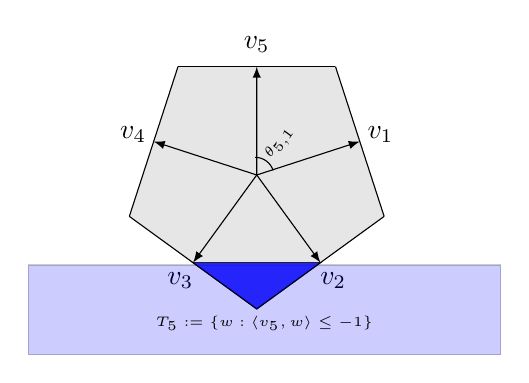
\begin{tikzpicture}[scale=2.0]
 \path[fill=gray, opacity=0.2] (0.95105651629,0.30901699437) coordinate(p1) --  ++(180:1) coordinate(p5)
 -- ++(252:1) coordinate(p4) --
 ++(324:1) coordinate(p3) --  ++(396:1) coordinate(p2);
 
 \coordinate (ctr) at (barycentric cs:p1=1,p2=1,p3=1,p4=1,p5=1);
 \foreach \X [count=\Y] in {2,...,6}
 {\ifnum\X=6
   \path (p\Y) -- (p1) coordinate[pos=0.0](a\Y) coordinate[pos=1.0](a1)
   coordinate[pos=0.5](m1);
   \draw (a\Y) -- (a1);
   \draw[-latex] (ctr) -- ($ (m1)!0.0cm!90:(p1) $) node[pos=1.2]{$v_{\Y}$};
  \else
   \path (p\Y) -- (p\X) coordinate[pos=0.0](a\Y) coordinate[pos=1.0](a\X)
   coordinate[pos=0.5](m\X);
   \draw (a\Y) -- (a\X);
   \draw[-latex] (ctr) -- ($ (m\X)!0.0cm!90:(p\X) $) node[pos=1.2]{$v_{\Y}$};
  \fi}
  \draw[fill=blue, opacity = 0.2] (-1.0,-0.95105) -- (-1.0,-1.52) -- (2.0,-1.52) -- (2.0,-0.95105) -- cycle;
  \node[rotate=54, xshift=0.5cm] at (ctr) {\tiny$\theta_{5,1}$};
  \draw (0.555, -0.35) arc (18:90:0.12);
  \node at (0.5,-1.32) {\tiny$T_5 := \{w : \langle v_5, w\rangle \leq -1 \}$};
  \draw[fill=blue, opacity = 0.8] (m3) -- (m4) -- (a3) -- cycle;
\end{tikzpicture}
\end{center}
\end{proof}

%%%% Previous versions of proofs:
%In fact, in order for the H-reps to be tight, we must observe that for all $i, j$, the $\max_{x \in S_i} \langle v_j, x \rangle = -1$ if $i = j$ and $1$ otherwise.
%For all $i,j$, we denote $x_{ij}$ so that $\langle v_i, x_{ij} \rangle = \langle v_j, x_{ij} \rangle = 1$.
%Numbering the normals clockwise (modulo 5), then for all $i$, we need $\langle v_i, x_{i+1, i+2} \rangle \leq -1$ and $\langle v_i, x_{i-1, i-2} \rangle \leq -1$.
%
%Focusing on $v_1$, we know that $\langle v_1, x_{23} \rangle \leq -1$ and $\langle v_1, x_{45} \rangle \leq -1$ if and only if $\theta_{13} = \theta_{12} + \theta_{23} \geq 180^o$  and $\theta_{41} = \theta_{51} + \theta_{45} \geq 180^o$.
%These statements are only jointly true if $\theta_{13} = \theta_{41} = 180^o$.
%However, the only way to reach this conclusion is if $\theta_{34} = 0^o$, and as the vectors are all unit vectors, we conclude $v_3 = v_4$.
%We can see that this scenario contradicts the tightness of the H-reps $(V, B_3)$ and $(V, B_4)$.
%As $S_3 = \{w : Vw \leq (1,1,-1,1,1)^T\}$, if $v_3 = v_4$, then the polytope $S_3$ is a line in $\reals^2$ and the constraint $\langle v_1, x \rangle = 1$ is not true for any $x \in S_3$.
%Therefore, there is some $i$ such that $(V,S_i)$ is not a tight H-representation.
%Thus, the cell $B^{(abs)}$ does not have a $2$-construction, and the property is not $2$-embeddable.


%Similarly, we can see that $\langle v_2, x_{34} \leq -1$ and $\langle v_2, x_{15} \rangle \leq -1$ if and only if $v_4 = -v_2$.
%Therefore, we know that $\theta_{24} = 180^o = \theta_{23} + \theta_{34} = \theta_{12} + \theta{51} + \theta_{45}$
%
%Now, in order for $\langle v_5, x_{12} \leq -1$ and $\langle v_2, x_{34} \rangle \leq -1$ to hold,
%
%Therefore, for all $v_i$, there must be some $v_j = -v_i$ in $V$.
%
%Consider $V = (v_1, \ldots, v_5)^T$ and, without loss of generality, let $v_1 = (0,1)$.
%
%
%We assert that $v_2 := -v_1$ must be in the set of normals.
%This can be seen since, for the normals $v_1$ and $v_2$, then angle $\theta_{12}$ between the two normals must be $180^o$.
%Since we have $5$ normals, the angle between normals $v_1$ and $v_2$ can be written $\theta{12} = \theta{1i} + \theta_{i2}$.
%(One direction of the angles must have some $v_i$ between $v_1$ and $v_2$.)
%If $\theta_{1i} \leq 90^o$, then $\theta_{1i} + \theta_{i2} \geq 180^o$ in order for there to be a $w$ such that $\langle v_2, w \rangle = 1$.
%
%
%\jessie{Left off here before the reading group}
%In order for the H-rep to be tight, then for all $v_j$ for $j > 1$, $\langle v_j, w \rangle = 1$ and $w = (x, -1)$.
%Observe that a line (here, a facet of the polytope) in $\reals^2$ cannot be non-redundantly bounded by $3$ points.
%This suggests that, in order for $(V,B_1)$ to be tight, at least two facets must both intersect $\langle v_1, w \rangle$ at the same point.
%However, since each $v_j$ must be a unit normal and the facets must intersect at the same point $w$, $\langle v_j, w \rangle = \langle v_k, w \rangle$ for $j \neq k$ if and only if $v_j = v_k$.
%However, if $v_j = v_k$, then the representations $(V, B_j)$ and $(V, B_k)$ will not be tight.
%This can be seen as there will be no $w \in \{ w: \langle v_j, w \rangle = 1 \}$ that is also on the face $\{w : \langle v_j, w \rangle =-1 \} = \{w : \langle v_k, w \rangle = -1\}$, and vice versa.
%Therefore, there is no set of normals $V \in \reals^{5\times 2}$ so that $\{w : Vw = B_i\}$ is tight for all $v_j$ and $B_i$.
%Therefore, since there is no $2$-construction of abstain(1/2) on $5$ outcomes, we conclude it is not $2$-embeddable.
%\jessie{Weird to think of it this way after drawing so many pictures, but this might be more elegant if it's close.}

\paragraph{On the matching upper bound.}
One cannot prove a better lower bound for abstain loss and $\reals^2$, as \citet{ramaswamy2018consistent} give a $2$-embedding for $|\Y|=4$.
This implies that a $2$-construction for the $4 \times 4$ version of the above $B$ matrix exists; and indeed, the above proof roughly reveals its shape.
One can take $V$ to be the four unit vectors pointing directly north, south, east, and west; the H-representations are then line segments, e.g. the segment $w_1=-1, w_2 \in [-1,1]$, etc.
These are all tight.
Indeed, as required by our characterization, the subgradient sets of their loss functions at the abstain embedding point span these H-reps (in fact are equal to them).

\bo{It would be nice to actually construct the losses for the ``rhombus'' and show that it embeds abstain loss. That might be a cool showcase for our understanding.}

\begin{theorem}
  Abstain with $\alpha > 1/2$ and $|\Y|=7$ is not $2$-embeddable.
\end{theorem}
\begin{proof}
  Like Theorem~\ref{thm:abs-5outcome-not-2embed}, we will again show that there is no $2$-construction of the abstain cell.
  First, note that when $\alpha \geq \frac{n-1}{n}$, the abstain property decomposes into the mode, as the abstain cell is empty, so we restrict to $\frac{n-1}{n} > \alpha > 1/2$.
  We then write the matrix $B$ describing the abstain cell as follows:
	\[ B = \begin{pmatrix}
       -\beta &  1 &  1 & \cdots & 1  \\
       1  & -\beta &  1 & \cdots & 1  \\
          &    &    & \vdots &    \\
       1  &  1 &  1 & \cdots & -\beta
     \end{pmatrix} .
  \]

  We know that $\beta := 1 - \frac{1}{\alpha} \in (0,1)$ as the inequalities describing $\alpha$ are strict.
  Observe that for all $i \in \{1,2, \ldots, 6\}, ||v_i|| > 0$.
  Additionally, we know $-\beta < 0$.
  Therefore, for all $i$, we know that $0 \not \in T_i$.
  By convexity of $T_i$ for all $i$, we then know that there is no line containing the origin in $T_i$.
  WLOG, as before, we say $v_1 = (0,1)$ and $||v_1|| \geq ||v_j||$ for all $j \neq 1$, we know that $\vec{0} \not \in T_1$.

  We assert that, in order for $(V, T_1)$ to be tight, then for all $j \neq i$, there must be a $w \in T_1$ such that $\inprod{v_j}{w} = 1$.
  However, in order for that to be true, $\theta_{1,j} > 60^o$. for all $j \neq 1$.
  Namely, $\theta_{1,2} > 60^o$, and $\theta_{6,1} > 60^o$.
  Observe that this argument is similar to the argument of Theorem~\ref{thm:abs-5outcome-not-2embed}.

  Applying the same argument iteratively, we know that if $v_c$ is the second-longest normal, in order for $(V, T_c)$ to be tight, we must observe $\theta_{c-1, c} > 60^o$ and $\theta_{c,c+1} > 60^o$.
  In fact, this argument must hold for each $\theta_j, j+1$.
  Additionally, we see for all $j$, that $\theta_{j,j+2} > 120^o$.
  However, since we know $\sum_{i=1}^6 \theta_{i,i+2} = 720$, and thus there must be some $\theta_{i,i+2} \leq 120$, yielding a contradiction.

  For the normals $v_i$ and $v_{i+2}$ such that $\theta_{i,i+2} \leq 120^o$, there is no way for the H-representation $(V, T_{i+1})$ to be tight. \jessie{justify...}

  Therefore, there is no $V$ yielding a $2$-construction for abstain on $6$ outcomes with $\alpha > 1/2$.
  (Like the triangle observed in the previous proof, we observe that, on the regular hexagon, $T_1$ is a trapezoid with some constraints that are not tight.)
\end{proof}

\paragraph{Implications.}
We conjecture that the construction of \citet{ramaswamy2018consistent} is optimal in all dimensions.
If so, this leaves two possibilities: It might be that there is some \emph{non-embedding} approach that elicits this property using a report space of fewer than $d=\lceil \log_2 |\Y|\rceil$ dimensions.
Going beyond the embedding approach seems to require new ideas that could be relevant to many applications in machine learning.
On the other hand, it might be that the best possible dimension is achieved by an embedding approach and polyhedral loss.
If true, it would be interesting to see how generally this might hold.
\begin{conjecture}\label{conj:abstain-tight}
  Abstain with $\alpha=1/2$ is $(\log_2 |\Y|)$-embeddable, but no lower.
\end{conjecture}

%%%%%%%%%%%%%%%%%%%%%%%%%%%%%%%%%%%%%%%%%%%%%%%%%%%%%%%%%%%%%%%
\section{Conclusion and Future Directions} \label{sec:conclusion}
\paragraph{Summary.}
This work is part of a broader research program to understand convex surrogates through the lens of property elicitation: the relationship between finite losses and convex surrogates, the link functions connecting them, and the properties they elicit.
We seek a general theory that, given a property, can prescribe when and how to construct convex surrogate losses that elicit it, and specifically, determine the minimum dimension required.
Even more broadly, one could replace ``convex'' by any notion of ``nice'' surrogate desired.

This work formalized the \emph{embedding} approach where labels are identified with points in $\reals^d$.
We saw \bo{in theorem ??} that this approach is tightly connected to the use of polyhedral (i.e. piecewise linear convex) loss functions.
We also saw that it is a general technique that can be used for any finite elicitable property.

We then investigated the \emph{dimensionality} of $\reals^d$ required for such embeddings, giving a characterization in terms of the structure of the property in the simplex.
This gave a complete understanding of the one-dimensional case, and a complete characterization albeit weaker understanding in higher dimensions.
%RF got here
The two key conditions are an optimality condition that relates the structure of each level set to existence of polytopes in $\reals^d$ satisfying certain conditions; and a monotonicity condition relating such polytopes for different level sets.
This yields new lower bounds in particular for the abstain loss.

\paragraph{Directions.}
There are several direct open questions involving embedding dimension.
It would be interesting and perhaps practically useful to develop further techniques for upper bounds: automatically constructing embeddings in $\reals^d$ and associated polyhedral losses from a given property, with $d$ as small as possible.
Another direction is additional lower bound techniques, or further development of our necessary conditions.

This paper also suggests an agenda of defining more nuanced classes of surrogate losses and studying their properties.
For example, a tangential topic in this work was the characteristics of a ``good'' link function; formalizing and exploring this question is an exciting direction.
We would also like to move toward a full understanding of the differences between these classes.
For example, how does embedding dimension compare in general to convex elicitation diemsnion (the dimensionality $d$ required of \emph{any} convex surrogate loss)?
These questions have both theoretical interest and potential practical significance.

\begin{conjecture}
  $\mathrm{elic}_{embed}(\Gamma) = \mathrm{elic}_{Pcvx}(\Gamma) = \mathrm{elic}_{cvx}(\Gamma)$ for all finite, elicitable properties $\Gamma$.
\end{conjecture}


\raf{ACKNOWLEDGEMENTS (commented out for submission)}
% \subsection*{Acknowledgements}
% We thank Peter Bartlett for several discussions early on, which led to a proof of \raf{1-d reduction} among other insights.
% \raf{Almost forgot: should ack Arpit too of course!}

\bibliography{diss,extra}

%%%%%%%%%%%%%%%%%%%%%%%%%%%%%%%%%%%%%%%%%%%%%%%%%%%%%%%%%%%%%%%
\appendix

%% Jessie commented out 1/31/19 because of the updated proof to the trim TFAE, these are now no longer necessary.
%%\section{Considering unlabeled properties}
%%  Note that when $\Gamma$ is elicitable, there is a convex score $G:\simplex \to \reals$ representing the Bayes Risk (i.e. $G(p)$ is the minimal expected loss over all reports at $p$.)
%%  There is a set $\D \subseteq \partial_p G$ so that there is a bijection $\phi:\D \to \R$.
%%  Therefore, the subgradients of $G$ correspond to the property value at the distribution $p$.
%%
%%  The next two proofs take advantage of this duality correspondence between the subgradients of the convex score $G$ of an elicitable property and the property values.
%%
%%
%%\begin{lemma}\label{lem:trim-subsets-not-full-dimensional}
%%Let $\Gamma:\simplex \toto \R'$ be an elicitable property.
%%For any $u,w \in \R'$, if $\Gamma_u \subsetneq \Gamma_w$, then $\Gamma_u$ is not full dimensional.
%%\end{lemma}
%%\begin{proof}
%%  If there is a full-dimensional level set $\Gamma_u \subsetneq \Gamma_w$, then the corresponding scoring rule $G$ must not be differentiable (i.e. $|\partial_p G(p)| > 1$) for all $p \in \Gamma_u$.
%%%  (This is true because $\phi^{-1}(u) \neq \phi^{-1}(w)$ as the level sets are not equal.)
%%  However, closed, convex, full-dimensional level sets have positive Lebesgue measure in $\reals^{n-1}$,\jessiet{I don't know if we need a citation/proof for this assertion...} and thus contradicts the convexity of $G$, as convex functions are differentiable at all but a countable set of points.
%%  This in turn contradicts the elicitability of $\Gamma$, and so, we conclude that $\Gamma_u$ is not full-dimensional.
%%\end{proof}
%%
%%\begin{lemma}\label{lem:unique-opt-on-inter}
%%  Let $\Gamma:\simplex \toto \R'$ be an elicitable property such that $\trim(\Gamma)$ is finite.
%%  For all $u \in \R'$, if $p \in \inter{\Gamma_u}$, then $\Gamma(p) = \{u\}$.
%%\end{lemma}
%%\begin{proof}
%%\jessiet{Come back and formalize}
%%  We'll use the relationship between non-redundant properties and subgradients of the expected score $G$.
%%  Now consider the following convex analysis fact: for any convex function and any two point which share a subgradient, the function is flat between those points.
%%  In particular, $G$ is flat on $\Gamma_u$, and therefore $G$ must be differentiable on the interior of $\Gamma_u$.
%%  Therefore, $G$ must only have one subgradient on $\inter{\Gamma_u}$.
%%  \bigskip
%%  \jessie{Formalization below}
%%  \hrule
%%  Consider that $\trim(\Gamma)$ is non-redundant, and $p \in \inter{\Gamma_u}$ only if $\Gamma_u \in \trim(\Gamma)$ by Lemma~\ref{lem:trim-full-dim}, as a closed, convex set is full-dimensional if and only if it has nonempty interior. \jessiet{Sanity check here?}
%%  Since $\Gamma$ is elicitable, the score $G$ must be convex.
%%  For $w \in \R'$, if $\Gamma_w \subseteq \Gamma_u$, then we contradict the nonredundancy of $\trim(\Gamma)$, so we only worry about the case where $\Gamma_w \not \subseteq \Gamma_u$..
%%
%%  Suppose there is such a level set.
%%  There must be another level set $v$ so that $\Gamma_w \cap \inter{\Gamma_v}$ is nonempty, since level sets of elicitable properties are closed.
%%  Therefore, for $q \in \Gamma_w$, we observe $\Gamma(q) \subseteq \{u,w\}$ or $\{v,w\}$.
%%  More importantly- for $q \in \Gamma_w$, $\Gamma(q)$ is not constant.
%%
%%  Let's say there is a $q \in \Gamma_w \cap \inter{\Gamma_u}$ and $q' \in \Gamma_w \cap \inter{\Gamma_v}$.
%%  Additionally, $\conv(\{q,q'\}) \subseteq \Gamma_w$, and observe that $\conv(\{q,q'\})$ is not countable.
%%  Since there is a bijection from $\Gamma(p)$ to $\partial_p G(p)$, we then note that $|\partial_pG(p)| > 1$ on an uncountable set, and $\partial_p G(p)$ is not constant on $\conv(\{q,q'\})$.
%%  This contradicts the convexity of $G$, and in turn, the elicitability of $\Gamma$ and $\trim(\Gamma)$.
%%
%%  Therefore, for all $p \in \inter{\Gamma_u}$, we must observe $\Gamma(p) = \{u\}$.
%%
%%\end{proof}
%%
%%\begin{corollary}\label{cor:cant-span-interiors}
%%  If $\Gamma:\simplex \toto \R'$ is a non-redundant, finite elicitable property, no level set spans the interior of two other level sets.
%%  Formally, there is no $w \in \R'$ so that for any $p \in \inter{\Gamma_u}$ and $q \in \inter{\Gamma_v}$, $p,q \in \Gamma_w$ for reports $u,v \in \R'$ with $u \neq v$.
%%\end{corollary}
%%\jessiet{I can write something for a proof of this if you want, but it follows from the previous statement pretty quickly.}
%%
%%\begin{lemma}\label{lem:trim-full-dim}
%%  Consider a nondegenerate, elicitable property $\Gamma$ with finitely many full-dimensional level sets.
%%  Every $\theta \in \Theta := \trim(\Gamma)$ is full-dimensional.
%%\end{lemma}
%%\begin{proof}
%%  Consider an arbitrary level set $\theta$.
%%  If $\theta$ is not full-dimensional, we want to show that it must be the intersection of some full-dimensional level sets in $\trim(\Gamma)$.\jessiet{Why?  Add more details about why the level set can't span two full-dimensional level sets}
%%  If it is a proper subset of the level sets of which it is the intersection, and so it is not in the $\trim$ as it is in the subtracted set.
%%
%%  Now suppose that a level set $\theta$ was not full-dimensional and not a proper subset of any one level set.
%%  It must then span the interior multiple level sets, as level sets of elicitable properties are closed.
%%  By Corollary~\ref{cor:cant-span-interiors}, we contradict the elicitability of $\Gamma$.
%%  Thus, any $\theta$ that is not full-dimensional must be the intersection of a finite set of full-dimensional level sets $\theta_i \in \trim(\Gamma)$.
%%  As trimming a property removes such redundant reports, we then observe that $\theta \not \in \trim(\Gamma)$.
%%  Therefore, each $\theta \in \trim(\Gamma)$ must be full-dimensional.
%%\end{proof}



%\begin{lemma}\label{lem:finite-nonred-fdls}
%Let $\Gamma:\simplex \toto \R'$ be a non-redundant, finite elicitable property.
%Each level set $\Gamma_u \in \{\Gamma_u : u \in \R' \}$ is full-dimensional.
%\end{lemma}
%\begin{proof}
%Let us consider 3 cases: first, we cannot observe a level set is a subset of or equal to another by nonredundancy of the property.
%Now, if one level set spans the interiors of two different level sets, we will see that this property is not elicitable.
%Since we assume $\Gamma$ is elicitable, we know the score $G$ is convex over $\simplex$.

%Now, suppose there are two distributions $q,q'$ such that $q \in \inter{\Gamma_u}$ and $q' \in \inter{\Gamma_{u'}}$ for $u \neq u'$.
%Additionally, if there is a report $w$ such that $\conv(\{q,q'\}) \subseteq \Gamma_w$, we say that the level set $\Gamma_w$ spans the interior of two level sets.

%First, consider that if $q \in \inter{\Gamma_u}$ and $q' \in \inter{\Gamma_{u'}}$ are two non-redundant points in the set $S$ such that $\Gamma_w = \conv(S)$, then there are distributions $p := q + \epsilon(q-q')$ and $p' = q' + \epsilon(q'-q)$ that are both in the interior of their respective level sets and $\Gamma(p) \cap \Gamma(p') = \emptyset$.
%By \jessie{Raf and Ian 2018} Lemma 10, then for $\lambda \in (0,1)$, the score $G(\lambda p + (1-\lambda) p') < \lambda G(p) + (1-\lambda) G(p')$.
%However, if $q$ and $q'$ share a subgradient, then the score $G$ is flat on $\conv(\{q,q'\})$, which is a subset of $\conv(\{p,p'\})$.
%However, this contradicts \jessie{Raf and Ian 2018} Lemma 10, as the score $G$ is flat (and therefore the strict inequality is actually an equality) on $(a,b) \subseteq (0,1)$.

%Now, if the level set $\Gamma_w$ is described as the convex hull of distributions $q \not \in \inter{\Gamma_u}$ or $q' \not \in \inter{\Gamma_{u'}}$, such distributions $p$ and $p'$ do not exist in the respective level sets.
%\jessie{.... other argument}

%Therefore, for the elicitable property $\Gamma$, there cannot be a level set $\Gamma_w$ that spans the interiors of two other level set.s

%\end{proof}

\section{To Sort}

Several definitions from \citet{aurenhammer1987power}.
\begin{definition}\label{def:cell-complex}
  A \emph{cell complex} in $\reals^d$ is a set $C$ of faces (of dimension $0,\ldots,d$) which (i) union to $\reals^d$, (ii) have pairwise disjoint relative interiors, and (iii) any nonempty intersection of faces $F,F'$ in $C$ is a face of $F$ and $F'$ and an element of $C$.
\end{definition}

\begin{definition}\label{def:power-diagram}
  Given sites $s_1,\ldots,s_k\in\reals^d$ and weights $w_1,\ldots,w_k \geq 0$, the corresponding \emph{power diagram} is the cell complex given by
  \begin{equation}
    \label{eq:pd}
    \cell(s_i) = \{ x \in\reals^d : \forall j \in \{1,\ldots,k\} \, \|x - s_i\|^2 - w_i \leq \|x - s_j\| - w_j\}~.
  \end{equation}
\end{definition}

\begin{definition}\label{def:affine-equiv}
  A cell complex $C$ in $\reals^d$ is \emph{affinely equivalent} to a (convex) polyhedron $P \subseteq \reals^{d+1}$ if $C$ is a (linear) projection of the faces of $P$.
\end{definition}

\begin{theorem}[\cite{aurenhammer1987power}]\label{thm:aurenhammer}
  A cell complex is affinely equivalent to a convex polyhedron if and only if it is a power diagram.
\end{theorem}

In particular, one can consider the epigraph of a polyhedral convex function on $\reals^d$ and the projection down to $\reals^d$; in this case we call the resulting power diagram \emph{induced} by the convex function.
We extend Aurenhammer's result to a weighted sum of convex functions, showing that the induced power diagram is the same for any choice of strictly positive weights.

\begin{lemma}\label{lem:polyhedral-pd-same}
  Let $f_1,\ldots,f_k:\reals^d\to\reals$ be polyhedral convex functions.
  The power diagram induced by $\sum_{i=1}^k p_i f_i$ is the same for all $p \in \inter\simplex$.
\end{lemma}
\begin{proof}
  For any convex function $g$ with epigraph $P$, the proof of~\citet[Theorem 4]{aurenhammer1987power} shows that the power diagram induced by $g$ is determined by the facets of $P$.
  Let $F$ be a facet of $P$, and $F'$ its projection down to $\reals^d$.
  It follows that $g|_{F'}$ is affine, and thus $g$ is differentiable on $\inter F'$ with constant derivative $d\in\reals^d$.
  Conversely, for any subgradient $d'$ of $g$, the set of points $\{x\in\reals^d : d'\in\partial g(x)\}$ is the projection of a face of $P$; we conclude that $F = \{(x,g(x))\in\reals^{d+1} : d\in\partial g(x)\}$ and $F' = \{x\in\reals^d : d\in\partial g(x)\}$.

  Now let $f := \sum_{i=1}^k f_i$ with epigraph $P$, and $f' := \sum_{i=1}^k p_i f_i$ with epigraph $P'$.
  By \raf{Rockafellar}, $f,f'$ are polyhedral.
  We now show that $f$ is differentiable whenever $f'$ is differentiable:
  \begin{align*}
    \partial f(x) = \{d\}
    &\iff \sum_{i=1}^k \partial f_i(x) = \{d\} \\
    &\iff \forall i\in\{1,\ldots,k\}, \; \partial f_i(x) = \{d_i\} \\
    &\iff \forall i\in\{1,\ldots,k\}, \; \partial p_i f_i(x) = \{p_id_i\} \\
    &\iff \sum_{i=1}^k \partial p_if_i(x) = \left\{\sum_{i=1}^k p_id_i\right\} \\
    &\iff \partial f'(x) = \left\{\sum_{i=1}^k p_id_i\right\}~.
  \end{align*}
  From the above observations, every facet of $P$ is determined by the derivative of $f$ at any point in the interior of its projection, and vice versa.
  Letting $x$ be such a point in the interior, we now see that the facet of $P'$ containing $(x,f'(x))$ has the same projection, namely $\{x'\in\reals^d : \nabla f(x) \in \partial f(x')\} = \{x'\in\reals^d : \nabla f'(x) \in \partial f'(x')\}$.
  Thus, the power diagrams induced by $f$ and $f'$ are the same.
  The conclusion follows from the obversation that the above held for any strictly positive weights $p$, and $f$ was fixed.
\end{proof}

\begin{theorem}\label{thm:general-duality-embedding}
  Let $\gamma:\simplex\toto\R$ be a non-redundant elicitable property, elicited by a loss whose Bayes risk is a closed function.
  Then $\gamma$ is $(n-1)$-embeddable, where $n=|\Y|$.
  \raft{Low priority: what conditions on $L$ or $\gamma$ ensure that the Bayes risk is closed?}
\end{theorem}
\begin{proof}
  $G:\simplex\to\reals$ be the negative Bayes risk of the loss $L_\gamma$ eliciting $\gamma$, given by $G(p) = -\min_{r\in\R} \inprod{p}{L_\gamma(r)}$.
  Let $C:\reals^\Y\to\reals$ be the convex conjugate of $G$, given by $C(u) = \sup_{p\in\simplex} \inprod{p}{u} - G(p)$, which is finite on all of $\reals^\Y$ by~\citet[Corollary 13.3.1]{rockafellar1997convex} as $\dom\, G = \simplex$ is bounded.

  By~\citet[Theorem 2]{frongillo2014general} we know that for some $\D \subseteq \partial G(\simplex) \subseteq \reals^\Y$ we have a bijection $s : \R \to \D$ such that $\gamma(p) = s^{-1}(\D \cap \partial G(p))$.
  (In other words, $\gamma$ is a relabeling of subgradients of $G$.)
  Thus, we can write
  \begin{equation}
    \label{eq:1}
    r \in \gamma(p) \iff s(r) \in \partial G(p) \iff p \in \partial C(s(r))~,
  \end{equation}
  where the final equivalence follows from~\cite[Corollary 23.5.2]{rockafellar1997convex} as $G$ is a closed convex function.

  Now define $L:\reals^n\to\reals^\Y$ by $L(u) = C(u)\ones - u$, where $\ones\in\reals^\Y$ is the all-ones vector.
  We will show that $L$ embeds $\gamma$.
  As $L$ is convex, we may write the optimality condition as
  \begin{equation}
    \label{eq:2}
    u \in \prop{L}(p) \iff u \in \argmin_{u'} \inprod{p}{L(u')} \iff 0 \in \partial \inprod{p}{L(u)}~,
  \end{equation}
  where the subgradient $\partial$ is with respect to $u$.
  Plugging in our definition of $L$, we have
  \begin{align*}
    0 \in \partial \inprod{p}{L(u)}
    & \iff 0 \in \partial \inprod{p}{\left(C(u)\ones - u\right)}
    \\
    % & \iff 0 \in \partial \left(C(u) - p\cdot u\right)
    % \\
    & \iff 0 \in \partial C(u) - \{p\}
    \\
    & \iff p \in \partial C(u)~.
  \end{align*}
  Together with eq.~\eqref{eq:1}, we now have for any $u \in \D$ and $p\in\simplex$ that
  \begin{equation}
    \label{eq:3}
    u \in \prop{L}(p) \iff p \in \partial C(u) \iff s^{-1}(u) \in \gamma(p)~.
  \end{equation}
  Recalling that $s$ is a bijection, we conclude that $L$ embeds $\gamma$ with embedding function $\varphi:\R\to\reals^\Y$ given by $\varphi(r) = s(r)$.

  We have now shown that $\gamma$ is $n$-embeddable.
  To drop a dimension, first note that $C$ is linear in the $\ones$ direction: for all $u'\in\reals^\Y$, the directional derivative $C'(u';\ones) = \sup_{p\in\partial C(u')} \inprod{p}{\ones} = 1$ as $\partial C(u')\subseteq\simplex$ for all $u'$; thus
  $C(u+\alpha\ones) = C(u) + \int_0^\alpha C'(u+\beta\ones;\ones) d\beta = C(u) + \alpha$.
  This linearity translates to invariance of $L$ in the direction of $\ones$:
  \begin{align*}
    L(u + \alpha\ones) = C(u+\alpha\ones)\ones - (u + \alpha\ones) = C(u)\ones + \alpha\ones - u - \alpha\ones = L(u)~.
  \end{align*}
  We now have for any $u\in\D$,
  \begin{align*}
    s^{-1}(u) \in \gamma(p) \iff u \in \prop{L}(p) \iff u - u_n\ones \in \prop{L}(p)\cap\R_2~.
  \end{align*}
  Letting $L':\reals^{n-1}\to\reals^\Y$ given by $L'(u') = L((u',0))$, and evoking Lemma~\ref{lem:loss-restrict}, we conclude $\prop{L'}(p) = \prop{L}\cap\R_2$ and thus $L'$ embeds $\gamma$ as well, with the embedding $\varphi(r) = (s(r)_1 - s(r)_n, \ldots, s(r)_{n-1} - s(r)_n)$.
  \jessiet{The notation $C'$ being a derivative kind of bothers me since $L'$ is used for another generic function... although I may just be misreading it or not familiar with standard notations.}
\end{proof}

\section{Dimension 1}\label{app:dimension-1}

\begin{definition}\label{def:monotone-prop}
  A property $\Gamma:\simplex\toto\R$ is \emph{monotone} if there are maps $a:\R\to\reals^\Y$, $b:\R\to\reals^\Y$ and a total ordering $<$ of $\R$ such that the following two conditions hold.
  \begin{enumerate}
  \item For all $r\in\R$, we have $\Gamma_r = \{p\in\simplex : \inprod{a(r)}{p} \leq 0 \leq \inprod{b(r)}{p} \}$.
  \item For all $r < r'$, we have $a(r) \leq b(r) \leq a(r') \leq b(r')$ (component-wise).
  % \item For all $r,r'\in\R$ and $p\in\Gamma_{r'}\setminus\Gamma_r$, we have $b(r) \cdot p < 0 \implies r' > r$ and $a(r) \cdot p > 0 \implies r' < r$.
  \end{enumerate}
\end{definition}

\begin{lemma}\label{lem:orderable-monotone}
  A finite property is orderable if and only if it is monotone.
\end{lemma}
\begin{proof}
  Let $\gamma:\simplex\toto\R$ be finite and monotone.
  Then we can use the total ordering of $\R$ to write $\R = \{r_1,\ldots,r_k\}$ such that $r_i < r_{i+1}$ for all $i \in \{1,\ldots,k-1\}$.
  We now have $\gamma_{r_i} \cap \gamma_{r_{i+1}} = \{p\in\simplex : \inprod{a(r_{i+1})}{p} \leq 0 \leq \inprod{b(r_i)}{p} \}$.
  If this intersection is empty, then there must be some $p$ with $\inprod{b(r_i)}{p} < 0$ and $\inprod{a(r_{i+1})}{p} > 0$; by monotonicity, no earlier or later reports can be in $\gamma(p)$, so we see that $\gamma(p) = \emptyset$, a contradiction.
  Thus the intersection is nonempty, and as we also know $b(r_i) \leq a(r_{i+1})$ we conclude $b(r_i) = a(r_{i+1})$, and the intersection is the hyperplane defined by $b(r_i) = a(r_{i+1})$.

  For the converse, let $\gamma:\simplex\toto\R$ be finite and orderable.
  From~\cite[Theorem 4]{lambert2018elicitation}, we have positively-oriented normals $v_i\in\reals^\Y$ for all $i \in \{1,\ldots,k-1\}$ such that $\gamma_{r_i} \cap \gamma_{r_{i+1}} = \{p\in\simplex : \inprod{v_i}{p} = 0\}$, and moreover, for all $i \in \{2,\ldots,k-1\}$, we have $\gamma_{r_i} = \{p\in\simplex : \inprod{v_{i-1}}{p} \leq 0 \leq \inprod{v_i}{p}\}$, while $\gamma_{r_1} = \{p\in\simplex : 0 \leq \inprod{v_1}{p} \}$ and $\gamma_{r_k} = \{p\in\simplex : \inprod{v_{k-1}}{p} \leq 0\}$.
  \jessiet{Should the sign on $\gamma_{r_k}$ be changed?}
  From the positive orientation of the $v_i$, we have for all $p\in\simplex$ that $\sgn(\inprod{v_i}{p})$ is monotone in $i$.
  In particular, it must be that for all $y$, $\sgn((v_i)_y)$ is monotone in $i$, taking the distribution with all weight on outcome $y$.
  % (Similarly, if $\gamma(\ones_y) = \{r_j,r_{j+1}\}$, then $(v_i)_y = v_i \cdot \ones_y < 0$ for $i < j$, $(v_j)_y = 0$, and $(v_i)_y > 0$ for $i > j$.)
  \raft{This observation could use a better proof.}

  For all $i\in\{2,\ldots,k-1\}$, we wish to find $\alpha_i \geq 0$ such that $v_{i-1} \leq \alpha_i v_i$ (component-wise).
  \jessiet{How should $w$ be interpreted?}
  To this end, fix $i$ and let $v = v_{i-1}, w = v_{i}, \alpha=\alpha_i$.
  By the above, there is no $y\in\Y$ with $v_y > 0 > w_y$, so the condition $v \leq \alpha w$ is equivalent to the following:
  \begin{enumerate}
  \item[(i)] For all $y$ with $v_y,w_y < 0$, $\alpha \leq v_y/w_y$.
  \item[(ii)] For all $y$ with $v_y,w_y > 0$, $\alpha \geq v_y/w_y$.
  \end{enumerate}
  Defining $\Y^- = \{y\in\Y: v_i,w_y < 0\}, \Y^+ = \{y\in\Y: v_i,w_y > 0\}$, these conditions are in turn equivalent to $\min_{y\in\Y^-} v_y/w_y \geq \max_{y\in\Y^+} v_y/w_y$, with the usual conventions $\min \emptyset = \infty,\; \max \emptyset = -\infty$.
  Suppose this inequality were not satisfied.
  Then we would have $y \in \Y^-,y'\in\Y^+$ such that $0 < v_y/w_y < w_{y'}/v_y$, which would in turn imply $|v_y|/v_{y'} < |w_y| / w_{y'}$.
  Letting $c = \tfrac 1 2 \left(|w_y| / w_{y'} + |v_y|/v_{y'}\right)$ and taking $p$ to be the distribution with weight $1/(1+c)$ on $y$ and $c/(1+c)$ on $y'$, we see that
  \begin{align*}
    \inprod{v}{p} &= \frac 1 {1+c} \left(v_y + \tfrac 1 2 (|w_y| / w_{y'} + |v_y|/v_{y'})v_{y'}\right) > \frac 1 {1+c} \left(v_y + (|v_y|/v_{y'})v_{y'}\right) = 0
    \\
    \inprod{w}{p} &= \frac 1 {1+c} \left(w_y + \tfrac 1 2 (|w_y| / w_{y'} + |v_y|/v_{y'})v_{y'}\right) < \frac 1 {1+c} \left(w_y + (|w_y|/w_{y'})w_{y'}\right) = 0~,
  \end{align*}
  thus violating the observation that $\sgn(\inprod{v_i}{p})$ is monotone in $i$ (recall that $v = v_{i-1}, w = v_{i}$).

  We can now construct the $a,b$ in Definition~\ref{def:monotone-prop}.
  Letting
  \[\alpha_i = \tfrac 1 2 \left(\min_{y\in\Y^-(i)} (v_{i-1})_y/(v_{i})_y + \max_{y\in\Y^+(i)} (v_{i-1})_y/(v_{i})_y\right)~,\] the preceding argument shows that $v_{i-1} \leq \alpha_i v_{i}$ for all $i \in \{2,\ldots,k-1\}$.
  We now set $b(r_i) = a(r_{i+1}) = (\prod_{j=2}^i \alpha_j) v_i$ for $i\in\{1,\ldots,k-1\}$, as well as $a(r_1) = -\max_{y\in\Y} |(v_1)_y|\ones$ and $b(r_k) = \max_{y\in\Y} |a(r_k)_y|\ones$, where $\ones\in\reals^\Y$ denotes the all-ones vector.

  The above establishes the second condition of monotone properties in Definition~\ref{def:monotone-prop}.
  To see the first condition, note that we have already established it for $i\in\{2,\ldots,k-1\}$.
  For $i=1,k$, we merely observe that $\inprod{a(r_1)}{p} \leq 0$ and $\inprod{b(r_k)}{p} \geq 0$ for all $p\in\simplex$.
\end{proof}

\raft{The following statement is true I believe, but low priority: ``An elicitable property $\Gamma:\simplex\toto\reals$ is convex elicitable (elicited by a convex $L : \reals \to \reals^\Y$) if and only if it is monotone.''  Start of the proof commented out.  Just need to show that $b$ is the upper limit of $a$ and $a$ the lower of $b$; should follow from elicitability of $\Gamma$.}
\begin{lemma}\label{lem:prop-L-monotone}
  For any convex $L : \reals \to \reals^\Y_+$, the property $\prop{L}$ is monotone.
\end{lemma}
\begin{proof}
  If $L$ is convex and elicits $\Gamma$, let $a,b$ be defined by $a(r)_y = \partial_- L(r)_y$ and $b(r) = \partial_+ L(r)_y$, that is, the left and right derivatives of $L(\cdot)_y$ at $r$, respectively.
  Then $\partial L(r)_y = [a(r)_y,b(r)_y]$.
  We now have $r \in \prop{L}(p) \iff 0 \in \partial \inprod{p}{L(r)} \iff \inprod{a(r)}{p} \leq 0 \leq \inprod{b(r)}{p}$, showing the first condition.
  The second condition follows as the subgradients of $L$ are monotone functions (see e.g.~\citet[Theorem 24.1]{rockafellar1997convex}).
  % Conversely, given such an $a,b$, we appeal to~\citet[Theorem 24.2]{rockafellar1997convex}, which gives us that $L(u)_y := \int_0^u a(u)_y$ is convex, and
\end{proof}

\newcommand{\Pbar}{\overline P}
\begin{lemma}\label{lem:pbar}
  Let $\gamma:\simplex\toto\R$ be a finite elicitable property, and suppose there is a calibrated link $\psi$ from an elicitable $\Gamma$ to $\gamma$.
  For each $r\in\R$, define $P_r = \bigcup_{u\in\psi^{-1}(r)} \Gamma_u \subseteq \simplex$, and let $\Pbar_r$ denote the closure of the convex hull of $P_r$.
  Then $\gamma_r = \Pbar_r$ for all $r\in\R$.
\end{lemma}
\begin{proof}
  As $P_r \subseteq \gamma_r$ by the definition of calibration, and $\gamma_r$ is closed and convex, we must have $\Pbar_r \subseteq \gamma_r$.
  Furthermore, again by calibration of $\psi$, we must have $\bigcup_{r\in\R} P_r = \bigcup_{u\in\reals} \Gamma_u = \simplex$, and thus $\bigcup_{r\in\R} \Pbar_r = \simplex$ as well.
  Suppose for a contradiction that $\gamma_r \neq \Pbar_r$ for some $r\in\R$.
  From Lemma~\ref{lem:finite-full-dim}, $\gamma_r$ has nonempty interior, so we must have some $p\in\inter\gamma_r \setminus \Pbar_r$.
  But as $\bigcup_{r'\in\R} \Pbar_{r'} = \simplex$, we then have some $r'\neq r$ with $p\in\Pbar_{r'} \subseteq \gamma_{r'}$.
  By Theorem~\ref{thm:aurenhammer}, the level sets of $\gamma$ form a power diagram, and in particular a cell complex, so we have contradicted point (ii) of Definition~\ref{def:cell-complex}: the relative interiors of the faces must not be disjoint.
  Hence, for all $r\in\R$ we have $\gamma_r = \Pbar_r$.
\end{proof}

We now prove the remaining results.
%Proposition~\ref{prop:indirect-orderable}, which states the following: if convex $L : \reals \to \reals^\Y$ indirectly elicits a finite elicitable property $\gamma$, then $\gamma$ is orderable.
\begin{proof}[of Proposition~\ref{prop:indirect-orderable}]
  Let $\gamma:\simplex\toto\R$.
  From Lemma~\ref{lem:prop-L-monotone}, $\Gamma := \prop{L}$ is monotone.
  Let $\psi:\reals\to\R$ be the calibrated link from $\Gamma$ to $\gamma$.
  From Lemma~\ref{lem:pbar}, we have $\Pbar_r = \gamma_r$ for all $r\in\R$, where $\Pbar_r$ is the closure of the convex hull of $\bigcup_{u\in\psi^{-1}(r)} \Gamma_u$.

  As $\Gamma$ is monotone, we must have $a,b : \R\to\reals^\Y$ such that $\Pbar_r = \{p\in\simplex : \inprod{a(r)}{p} \leq 0 \leq \inprod{b(r)}{p} \}$.
  (Take $a(r)_y = \inf_{u\in\psi^{-1}(r)} a(u)_y$ and $b(r)_y = \sup_{u\in\psi^{-1}(r)} b(u)_y$.)
  Now taking $p_r\in\inter\gamma_r$ and picking $u_r \in \Gamma(p_r)$, we order $\R = \{r_1,\ldots,r_k\}$ so that $u_{r_i} < u_{r_{i+1}}$ for all $i\in\{1,\ldots,k-1\}$.
  (The $u_{r_i}$ must all be distinct, as we chose $p_r$ so that $\gamma(p_r) = \{r\}$, so $\psi(u_{r_i}) = r_i$ for all $i$.)

  Let $i\in\{1,\ldots,k-1\}$.
  By monotonicity of $\Gamma$, we must have $a(r_i) \leq b(r_i) \leq a(r_{i+1}) \leq b(r_{i+1})$.
  As $\bigcup_{r\in\R} \Pbar_r = \bigcup_{r\in\R} \gamma_r = \simplex$, we must therefore have $b(r_i) = a(r_{i+1})$.
  Finally, we conclude $\gamma_{r_i} \cap \gamma_{r_{i+1}} = \{p\in\simplex : \inprod{b(r_i)}{p} = 0\}$.
  As these statements hold for all $i\in\{1,\ldots,k-1\}$, $\gamma$ is orderable.
\end{proof}

\newcommand{\floor}[1]{\lfloor #1\rfloor}
\begin{proof}[of Theorem~\ref{thm:1d-tfae}]
  As remarked before the theorem statement, it remains only to show $1 \iff 5$.
  \raft{This got a tad hand-wavy toward the end, but I think it's not too bad.}
  For the forward direction, by Lemma~\ref{lem:orderable-monotone}, we have $v(0),\ldots,v(k)\in\reals^\Y$ such that the coefficients $v(i)_y$ are monotone in $i$ for all $y\in\Y$, and the following two conditions hold: (1) for all $i\in\{1,\ldots,k\}$ we have $\gamma_{r_i} = \{p\in\simplex : \inprod{v(i-1)}{p} \leq 0 \leq \inprod{v(i)}{p} \}$, and (2) for all $i\in\{1,\ldots,k-1\}$ we have $\gamma_{r_i} \cap \gamma_{r_{i+1}} = \{p\in\simplex : \inprod{v(i)}{p} = 0\}$.
  Letting $\floor{u}$ denote the floor function, and $\mathrm{mod}(u) := u - \floor{u}$, we extend the above definition to $v:[0,k]\to\reals^\Y$ given by
  \begin{align*}
    v(u) = (1-\mathrm{mod}(u))v(\floor{u}) + \mathrm{mod}(u)v(\floor{u}+1)~,
  \end{align*}
  which is continuous by construction.
  Moreover, $v(\cdot)_y$ is monotone for all $y\in\Y$.
  As the level sets $\gamma_r$ are full-dimensional (Lemma~\ref{lem:finite-full-dim}), for all $p\in\simplex$, there is a unique $u\in[0,k]$ such that $\inprod{v(u)}{p} = 0$.
  We conclude that the property $\Gamma:\simplex\to[0,k]$ given by $\Gamma_u = \{p\in\simplex : \inprod{v(u)}{p} = 0\}$ is a single-valued property, which continuous as $v$ is continuous.
  Finally, the link $\psi(u) = \floor{u}+1$ is calibrated from $\Gamma$ to $\gamma$.

  For the converse, let $\Gamma:\simplex\to\reals$ be a continuous, non-locally-constant, elicitable property, with a calibrated link $\psi:\reals\to\R$ to $\gamma$.
  By~\cite{lambert2018elicitation,steinwart2014elicitation}, we have some continuous $v:\Gamma(\simplex)\to\reals^\Y$ such that for all $u\in\Gamma(\simplex)$ we have $\Gamma_u = \{p\in\simplex : \inprod{v(u)}{p} = 0\}$.

  Let $c_r = \inf\psi^{-1}(r)$ and $d_r = \sup \psi^{-1}(r)$ for all $r\in\R$, and let $I_r = (c_r,d_r)$.
  By continuity, $\Gamma^{-1}(I_r)$ is an open set, and the definition of calibration, we have $\Gamma^{-1}(I_r) \subseteq \gamma_r$; we conclude $\Gamma^{-1}(I_r) \subseteq \inter\gamma_r$.
  Again by continuity of $\Gamma$, we must have $\Gamma(\gamma_r) = [c_r,d_r] := \overline I_r$.

  As the interiors of the level sets of $\gamma$ are disjoint (Theorem~\ref{thm:aurenhammer}), the intervals $\{I_r:r\in\R\}$ must also be disjoint.
  Define an ordering $\R = \{r_1,\ldots,r_k\}$ so that $I_{r_1} < \cdots < I_{r_k}$.
  Then for all $i\in\{1,\ldots,k-1\}$ we must have $d_{r_i} = c_{r_{i+1}}$; otherwise, the point $u = \tfrac 1 2 (d_{r_i} + c_{r_{i+1}})$ would not belong to any $\overline I_r$, and as $\Gamma(\simplex) = \Gamma(\bigcup_r\gamma_r) = \bigcup_r \overline I_r$, this would violate continuity of $\Gamma$.
  We conclude that $\gamma_{r_i}\cap\gamma_{r_{i+1}} = \Gamma_{d_i} = \{p\in\simplex : \inprod{v(d_i)}{p} = 0\}$ for all $i\in\{1,\ldots,k-1\}$.
\end{proof}



\end{document}
%%% Local Variables:
%%% mode: latex
%%% TeX-master: t
%%% End:
